% !TEX root = diss.tex

\chapter{Interrogation of the Bell-Evans-Polanyi Principle: Investigation of the Bond Dissociation Enthalpies correlated with Hydrogen Atom Transfer Rate Constants}
\label{ch:bde}

\section{Introduction}

The Bell-Evans-Polanyi (BEP) principle is a conceptual framework that states, for two closely related reactions, the difference in activation energy is proportional to the difference in their enthalpy of reaction.\cite{Bell1936,Evans1938,Dill2003} This is commonly expressed as the linear free energy relationship in Equation 1.1 \jnote{Introduction}. Initially, the BEP principle was used as a simple model to explain the Br{\o}nsted catalysis law, which states that the stronger and acid is, the faster the catalysed reaction will proceed.\cite{Bronsted1924} A key assumptions is made for the BEP principle: the position of the TS along the reaction coordinate is the same for all reactions. The relationship can be described schematically: the more stable the product, the lower the reaction barrier, as seen in~\ref{fig:bep}.

\begin{figure}[htb]
  \centering
  
\includegraphics[width=0.7\textwidth]{figures/bep}
  \caption{Energy profiles for a series of related exothermic reactions illustrating the Bell-Evans-Polanyi principle.}
\label{fig:bep}
\end{figure}

A modern use of the BEP principle is to estimate rate constants of related reactions. If the relationship holds for a series of related HAT reactions, then bond dissociation enthalpies (BDEs) should correlate with the activation energy, and thus through the Arrhenius equation, rate constants. For instance, an increase in bond strength would represent a destabilisation in the TS complex, and thus a decrease in reaction rate. In application, plots of the logarithm of the rate constant, $k$, against BDEs are used. An interesting example of this is the work of \citet{Pratt2003}, in which the free radical oxidation of unsaturated lipids was examined. They demonstrate the correlation of theoretically determined allylic or benzylic C-H and \ch{C-OO^.} bond strengths with experimentally measured HAT rate constants and \ch{O2} addition rate constants, respectively. BEP plots ($\log k$ vs. BDE) for a large range of polyunsaturated fatty acid models show good correlation for \ch{C-OO^.} bonds examined, and reasonable correlation for \ch{C-H} bonds. This demonstrates that BDEs have a direct impact on the reaction barrier height, thus providing validation of the BEP principle. Importantly, these results also provide a means for predicting rate constants of related HAT and oxygen addition reactions by means of calculating BDEs.

\jnote{Expand this section}
A major problem is the lack of applicability criterion for how broadly the BEP principle can be utilised. In this work, I explore this issue. In order to achieve this, I examine HAT reactions involving the abstraction of C-H bonds by \cumo, for which many rate constants have been published.\cite{Bietti2010, Bietti2011, Pischel2001, Salamone2011, Salamone2012, Salamone2012a, Salamone2013, Salamone2015} Additional unpublished rate constants have been provided by our experimental colleagues in Rome. We have hypothesised that there should exist two distinct BEP relations: one in which the incipient radical is delocalised into a $\pi$-system (benzylic or allylic), and the remaining alkyl radicals which are largely localised.


BDEs are measurable using a large number of different experimental techniques, and a great deal of data exists in the literature. Much of this data has been compiled in the \emph{de facto} reference for BDEs: the CRC Handbook of Bond Dissociation Enthalpies.\cite{Luo2002} However, caution must be taken with experimentally determined BDEs, as not all experimental methods give reliable data. For example, BDEs from the Bordwell\cite{Bordwell1988} thermochemical cycle are possibly unreliable.\cite{Salamone2012, Miller2016} This was demonstrated for the BDE of dimethyl sulfoxide (DMSO), for which the experimentally determined BDE is about 8 \kcalmol lower than the best computational estimate.\cite{Salamone2012} Therefore, quantum chemistry is a useful tool for studying BDEs, as it is facile to compute BDEs. For example, an arbitrary \ch{X-H} bond strength is given by:

\begin{equation}
  \Delta H(BDE) =  H(\ch{X^.}) + H(\ch{H^.}) - H(\ch{X-H})
\end{equation}

\noindent where $\Delta H(BDE)$ is the BDE, and the right-hand terms are the enthalpies of the incipient radical, the hydrogen atom, and the substrate, respectively.

DFT-based methods have been shown to give reliable relative BDEs, however, highly correlated wave function based methods are required to predict chemically accurate (sub-\kcalmol) BDEs.\cite{DiLabio1999, Chan2012, Wiberg2014} For this purpose, we shall use composite quantum chemical procedures. Unfortunately, due to the computational cost of some of these procedures, calculations are often limited to small molecules. Additionally, there is currently no literature which compares the ability of common composite methods to predict accurate BDEs. Therefore, another aim of the work is to determine which composite procedure can be used to compute accurate BDEs for relatively large molecules.

\section{Methods}

Experimental rate constants were have either provided from unpublished results from our colleagues, the Bietti group in Rome, or come from literature sources.\cite{Bietti2010, Bietti2011, Pischel2001, Salamone2011, Salamone2012, Salamone2012a, Salamone2013, Salamone2015} All rate constants come from laser flash photolysis (LFP) experiments of \cumo~ with the substrates of interest. Acetonitrile solvent and ambient conditions (298 K and 1 atm) were used in all cases. For those results which have are unpublished, \cumo~ is generated by laser pulses at either 266 nm or 355 nm in solutions of excess dicumyl peroxide. Many of the literature results are also from the Bietti group, where the same procedure is used. Other results may have small variations in experimental details, however, all results are well time-resolved.

Observed rate constants ($k_{obs}$) are obtained from transient absorption decay traces of \cumo monitored at 485 nm. The observed rate constant is plotted against concentration of substrate to provide the bimolecular HAT rate constant ($k_H$) as the slope ($k_{obs} = k_0 + k_H[substrate]$). The \cumo radical decays unimolecularly through the $\beta$-scission of a methyl group, giving acetophenone and a methyl radical, as shown in~\ref{fig:cumo-decay}. The unimolecular decay rate constant\cite{Avila1995} for \cumo ($k_0$) in acetonitrile is on the order of 7.5 \E{5} s$^{-1}$.

\begin{scheme}[h!]
  \centering
  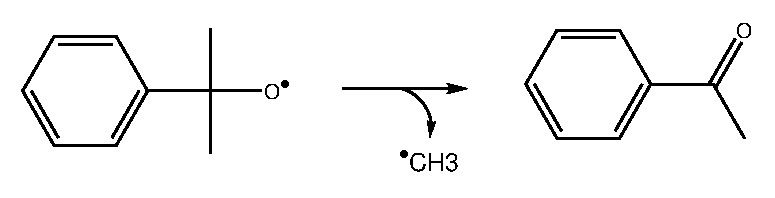
\includegraphics[width=0.75\textwidth]{figures/cumobeta.eps}
\caption{Unimolecular decay of the cumyloxyl radical.}
\label{fig:cumo-decay}
\end{scheme}

All quantum chemical calculations were performed using the Gaussian 09 software package.\cite{Frisch2009} Several composite quantum chemical method which are implemented in Gaussian 09 were used in this work: W1BD, CBS-QB3 and the restricted open-shell variant ROCBS-QB3, CBS-APNO, and G4 and the MP2 variant G4(MP2). An approach using ROCCSD(T) with locally-dense basis sets\cite{DiLabio1999LDBS, Wright2001} (LDBS) was also utilised in order to approximate W1BD results. Each of these methods is briefly described below.


\subsection{Quantum chemical composite procedures}

\noindent \textbf{W1BD}

The highest accuracy method used is W1BD, which employs seven different calculations to obtain highly correlated electronic energies, as well as thermochemically corrected quantities. This method is very computationally expensive, and thus cannot be applied to the larger species of interest in this work. Geometries and thermochemical corrections come from DFT-based B3LYP calculations with nearly complete cc-pVTZ+d basis sets. A frequency scaling factor of 0.985 is used for harmonic frequency calculations. The electronic energy comes from several additive corrections involving the Brueckner Doubles\cite{Barnes2009} (BD) variation of coupled cluster and various large basis sets extrapolated to the complete basis set limit. Corrections for core-electron correlation and relativistic contributions are computed using an uncontracted variant of the cc-pVTZ+2df basis sets, known as MTsmall.\cite{Martin1999}
\\

\noindent \textbf{LDBS approach}

Locally-dense basis sets have been used in the past to calculated BDEs for relatively large molecules.\cite{DiLabio1999LDBS, Wright2001} The principle is to use large basis sets to treat the atoms in which chemistry takes place, and use progressively smaller basis sets for ``remote'' portions of the molecule. We chose a method which best approximate W1BD results for a small subset of molecules. The scheme utilised herein obtains geometries and scaled thermochemical corrections from DFT-based B3LYP/cc-pVTZ+d, as used in the W1BD procedure. Single-point energy calculations were then performed using ROCCSD(T) and an LDBS partitioning scheme demonstrated in~\ref{fig:ldbs}, which uses the polarisation consistent basis sets.\cite{Jensen2001}

\begin{scheme}[!ht]
\centering
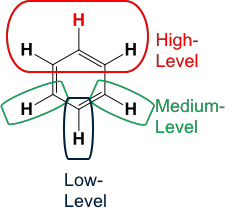
\includegraphics[width=0.75\textwidth]{figures/ldbs}
\caption[Locally-dense basis set partitioning used in the calculation of BDEs.]{Locally-dense basis set partitioning used in the calculation of BDEs. The scheme is referred to as pc-3/3/2/1, where for the shown benzene molecule, the centre of \ch{C-H} cleavage and the immediately adjacent groups are treated with high-level pc-3 basis sets. The next groups are treated with medium level pc-2 basis sets, and all other atoms are treated with low-level pc-1 basis sets.}
\label{fig:ldbs}
\end{scheme}

\noindent \textbf{CBS methods}

The Complete Basis Set (CBS) methods of Petersson and coworkers\cite{Montgomery1999, Montgomery2000, Ochterski1996, Wood2006} are widely used because of the relatively low computational cost (compared to other composite procedures), and well established accuracy.\cite{Somers2015, Simmie2015} CBS-QB3\cite{Montgomery1999, Montgomery2000} utilises DFT-based B3LYP optimisation and scaled frequencies (factor = 0.990) with modified triple-zeta Pople style basis sets. Electronic energies are obtained by extrapolation of medium basis set CCSD(T) and MP4SDQ. Small empirical corrections for are added to achieve more accurate results compared to the parametrisation sets.\cite{Petersson2001} ROCBS-QB3 is a similar procedure to CBS-QB3, except spin-resticted wave functions are used in place of unrestricted wave functions. This is done to eliminate spin contamination, and the use of an restricted open-shell definition has been shown to produce more accurate BDEs.\cite{DiLabio1999} (RO)CBS-QB3 has been implemented for first, second, and third periods of elements.

Atomic pair natural orbital (APNO) expansions are a method used for averaging over multiple Slater determinants. The use of APNOs allows for small basis set extrapolation of higher order correlation energies to converge more rapidly to the complete basis set limit. This approach is used in the CBS-APNO method.\cite{Ochterski1996} Geometries and scaled frequencies (factor = 0.989) are obtained at the QCISD/6-311G(d,p) level of theory. Similar to CBS-QB3, the extrapolation of moderate basis set MP4SDQ and QCISD(T) results gives the electronic energy. An empirical correction is also used in CBS-APNO. Even though CBS-APNO is more accurate, the expansion of APNOs makes CBS-APNO more computationally demanding than CBS-QB3. As a results, it has only been implemented for first and second row periods, and is thus less commonly used in literature.
\\

\noindent \textbf{G$n$ methods}

The Gaussian$-n$ (G$n$) series of methods originate from the Pople group,\cite{Pople1989} where G4 is the fourth generation. G4 utilises moderately large basis sets and extrapolation techniques with CCSD(T) calculations to obtained highly correlated electronic energies. G4(MP2) uses MP2 in place is CCSD(T) and is thus less computationally expensive, but also gives a less complete description of electron correlation. Both methods use the B3LYP/6-31(2df,p) level of theory for optimisation and frequency calculations with a frequency scaling factor of 0.9854. G4 results have been described as generally on par with CBS-QB3 results,\cite{Somers2015, Simmie2015} but calculations are more computationally expensive.

\subsection{Transition state calculations}

Calculations were performed to identify the lowest energy TS complex of several reactions between \cumo~ and organic substrates. In all cases cisoid and transoid conformations were explored. All optimisation calculations were performed at the B3LYP-D3(BJ)/6-31+G$^*$ level of theory. Single-point energy calculation were carried out at the LC-$\omega$PBE-D3(BJ)/6-311+G(2d,2p) level of theory.

\section{Comparison of composite method for the prediction of BDEs}
\jnote{Convince ROCBS-QB3 is best}
In order to determine the best method for BEP principle analysis, and to investigate which is the most efficient yet accurate composite method, the BDEs of 49 species have been calculated. This set of species contains a wide variety of chemical functionalities, thus this set may be described as a comprehensive test of these methods for C-H BDEs. Given that W1BD is the most accurate method used, these results have been used for comparison to other composite method. Unfortunately, BDEs for only 33 out of the 49 species studied were able to be calculated using W1BD due to computational cost restrictions: hard disk capacity was insufficient for large systems. Therefore, literature BDEs from \citet{Luo2002} for all species in the set are also used for comparison. The literature and calculated BDEs are listed in~\ref{tab:bde-calc}.

\begin{landscape}
%\singlespacing
\begin{longtable}{m{3.1cm} | c c c c c c c c}
\caption[Bond dissociation enthalpies of the species used to investigate the accuracy of composite methods.]{Bond dissociation enthalpies of the species used to investigate the accuracy of composite methods. All values are in \kcalmol. Statistics are listed at the bottom of the table.} \label{tab:bde-calc} \\
Molecule                         &  Lit.\cite{Luo2002}      &   W1BD   &     LDBS &     CBS-QB3 &   ROCBS-QB3 &   CBS-APNO &    G4   &    G4(MP2)\\
\hline
\endfirsthead
Molecule                         &  Lit.\cite{Luo2002}      &   W1BD   &     LDBS &     CBS-QB3 &   ROCBS-QB3 &   CBS-APNO &    G4   &    G4(MP2)\\
\hline
\endhead
1,3-pentadiene                   &  83.0     &   82.9   &   82.2   &    80.9     &    81.7    &   81.8   &  81.6   &    82.1   \\
1,4-diazabicyclo[2.2.2]-octane   &  93.4     &          &   98.9   &    98.9     &    98.8    &   98.5   &  96.7   &    95.6   \\
1,4-pentadiene                   &  76.6     &   76.2   &   76.0   &    74.2     &    75.0    &   75.2   &  75.1   &    75.7   \\
2,2-dimethylbutane               &  98.0     &   99.3   &   99.1   &    99.4     &    99.3    &   99.7   &  97.5   &    96.7   \\
2,3-dimethylbutane               &  95.4     &   97.8   &   97.7   &    97.9     &    97.8    &   98.0   &  96.2   &    95.5   \\
2-methylbutane                   &  95.8     &   97.3   &   97.2   &    97.3     &    97.1    &   97.3   &  95.9   &    95.5   \\
Acetaldehyde                     &  94.3     &   95.9   &   95.3   &    95.3     &    95.7    &   95.5   &  94.9   &    94.8   \\
Acetone                          &  96.0     &   96.9   &   96.4   &    96.2     &    96.7    &   97.1   &  95.4   &    95.0   \\
Acetonitrile                     &  97.0     &   96.9   &   96.6   &    96.2     &    96.6    &   96.5   &  96.3   &    96.3   \\
Adamantane (2$^\circ$)           &  98.4     &          &  100.9   &   100.5     &   100.4    &  100.9   &  97.8   &    96.3   \\
Adamantane (3$^\circ$)           &  96.2     &          &  100.3   &    99.9     &    99.9    &  100.3   &         &    95.7   \\
Benzaldehyde                     &  88.7     &          &   90.9   &    91.5     &    91.4    &   91.0   &  89.3   &    88.2   \\
Benzene                          & 112.9     &  113.1   &  112.7   &   115.4     &   113.0    &          &         &   113.0   \\
Benzyl Alcohol                   &  79.0     &          &   84.4   &    84.3     &    83.2    &   83.9   &  83.4   &    83.6   \\
Cumene                           &  83.2     &          &   87.9   &    87.9     &    86.9    &          &  86.9   &    86.7   \\
Cycloheptane                     &  94.0     &          &   96.0   &    96.0     &    95.8    &   96.1   &  93.9   &    92.9   \\
Cyclohexadiene                   &  76.0     &   76.3   &   76.2   &    74.3     &    75.0    &          &  75.2   &    75.5   \\
Cyclohexane                      &  99.5     &   99.2   &   99.1   &    99.4     &    99.3    &   99.6   &  97.5   &    96.8   \\
Cyclooctane                      &  94.4     &          &   92.6   &    92.6     &    92.4    &   92.8   &  90.2   &    89.1   \\
Cyclopentane                     &  95.6     &   96.3   &   96.1   &    96.5     &    96.3    &   96.6   &  95.6   &    95.0   \\
Cyclopropane                     & 106.3     &  109.0   &  108.5   &   109.3     &   109.2    &  109.5   & 108.2   &   108.0   \\
Dibenzyl ether                   &  85.8     &          &   83.6   &    84.3     &    82.7    &          &         &    79.6   \\
Diethyl ether                    &  93.0     &   95.3   &   95.1   &    95.6     &    95.5    &   95.4   &  93.8   &    93.1   \\
Dihydroanthracene                &  76.3     &          &   80.4   &    80.9     &    78.1    &          &         &    79.9   \\
Dimethylamine                    &  94.2     &   92.6   &   92.4   &    92.9     &    92.8    &   92.7   &  92.0   &    91.9   \\
Dimethylsulfoxide                &  94.0     &  102.0   &  101.7   &   102.3     &   102.3    &          & 100.9   &   100.6   \\
Dioxane                          &  96.5     &   97.3   &   97.3   &    97.7     &    97.6    &   97.4   &  95.7   &    94.9   \\
Diphenylmethane                  &  84.5     &          &   84.1   &    85.3     &    82.8    &          &         &    84.5   \\
Ethane                           & 100.5     &  101.3   &   99.3   &   101.7     &   101.5    &  101.8   & 100.7   &   100.7   \\
Ethylbenzene                     &  85.4     &          &   88.3   &    88.6     &    87.6    &   89.3   &  87.6   &    87.7   \\
Ethylene                         & 110.9     &  110.8   &  110.3   &   110.6     &   110.9    &  111.1   & 109.9   &   110.2   \\
Fluorene                         &  82.0     &          &   82.4   &    83.6     &    81.9    &          &         &    81.2   \\
Formaldehyde                     &  88.0     &   88.6   &   88.0   &    89.1     &    88.9    &   88.2   &  88.2   &    87.9   \\
Hexamethyl-phosphoramide         &           &          &   93.8   &    94.1     &    93.9    &          &         &    88.5   \\
Indene                           &  83.0     &          &   80.6   &    80.4     &    80.1    &   81.2   &  79.0   &    78.3   \\
Methane                          & 105.0     &  105.0   &  104.4   &   105.4     &   105.2    &  105.4   & 104.5   &   104.6   \\
Methanol                         &  96.1     &   96.4   &   96.0   &    96.9     &    96.8    &   96.6   &  96.0   &    95.8   \\
Methylamine                      &  93.9     &   93.1   &   92.8   &    93.4     &    93.3    &   93.3   &  92.7   &    92.8   \\
Morpholine                       &  92.0     &          &   93.4   &    93.4     &    93.3    &   93.3   &  91.8   &    91.1   \\
N,N-dimethylacetamide (acetyl)   &  91.4     &   99.6   &   99.4   &    99.5     &    99.5    &  100.1   &  97.6   &    96.8   \\
Piperazine                       &  93.0     &   93.4   &   93.5   &    93.6     &    93.5    &   93.4   &  91.9   &    91.2   \\
Piperidine                       &  89.5     &   92.1   &   92.2   &    92.3     &    92.2    &   92.1   &  90.7   &    90.0   \\
Propane                          & 100.9     &  101.6   &  101.3   &   102.0     &   101.8    &  102.1   & 100.7   &   100.4   \\
Pyrrolidine                      &  89.0     &   90.8   &   90.6   &    90.8     &    90.7    &   90.7   &  89.5   &    89.0   \\
Tetrahydro-2H-pyran              &  96.0     &   96.3   &   96.2   &    96.6     &    96.5    &   96.3   &  94.7   &    93.9   \\
Tetrahydrofuran                  &  92.1     &   93.7   &   93.3   &    93.9     &    93.8    &   93.6   &  92.2   &    91.6   \\
Toluene                          &  89.7     &   90.5   &   90.1   &    90.6     &    89.7    &   91.9   &  89.8   &    90.2   \\
Trichloromethane                 &  93.8     &   93.5   &   93.4   &    93.8     &    93.7    &          &  92.4   &    92.0   \\
Triethylamine                    &  90.7     &          &   91.4   &    91.3     &    91.2    &   91.4   &  89.4   &    88.4   \\
Trifluormethane                  & 106.4     &  107.2   &  106.6   &   107.4     &   107.4    &  106.8   & 105.8   &   105.0   \\
\hline
\textbf{Statistics}             & Lit.       &  W1BD    &    LDBS  &    CBS-QB3  &  ROCBS-QB3  &  CBS-APNO &    G4  &    G4(MP2)\\
\hline
Number of BDEs ($N$) &    49     &     33   &     50   &      50     &      50     &     40    &    43   &     50   \\
MAE (Lit.)                       &           &   0.82   &   1.60   &    1.88     &    1.64     &   1.35    &  1.21   &   1.57   \\
Max. Error                             &           &   1.59   &   2.41   &    2.63     &    3.15     &   1.85    &  4.19   &   6.23   \\
Min. Error                           &           &  -8.22   &  -8.04   &   -8.26     &   -8.25     &  -8.74    & -6.86   &  -6.58   \\
MAE (W1BD)                       &           &          &   0.22   &    0.32     &    0.18     &   0.20    &  0.70   &   0.88   \\
Max. Error                            &           &          &   2.00   &    2.01     &    1.26     &   1.08    &  2.05   &   2.84   \\
Min. Error                            &           &          &  -0.09   &   -2.37     &   -0.35     &  -1.39    &  0.37   &   0.02   \\
\end{longtable}

\end{landscape}

Mean absolute error (MAE) is used to assess the quality of computational methods, with errors calculated with respect to benchmark values for a given data set.\cite{Savin2014} The MAE is calculated as

\begin{equation}
  \mathrm{MAE} = \frac{1}{N} \sum | E_{ref} - E_{calc}|
\end{equation}

\noindent where for a set of $N$ reference values, the MAE is the average of the mean differences of the reference energy ($E_{ref}$) and the calculated value ($E_{calc}$). The MAE with respect to W1BD and literature shall be reported herein as ``MAE$_{\mathrm{W1BD}}$ (MAE$_{\mathrm{Lit.}}$)''. An additional semi-quantitative metric which I used to evaluate the accuracy of composite procedures to reproduce experimental results, is a bar chart which summarises the number of deviations from literature within given error ranges. This bar chart is reported in~\ref{fig:maebarchart}

\begin{figure}[htb]
  \centering
  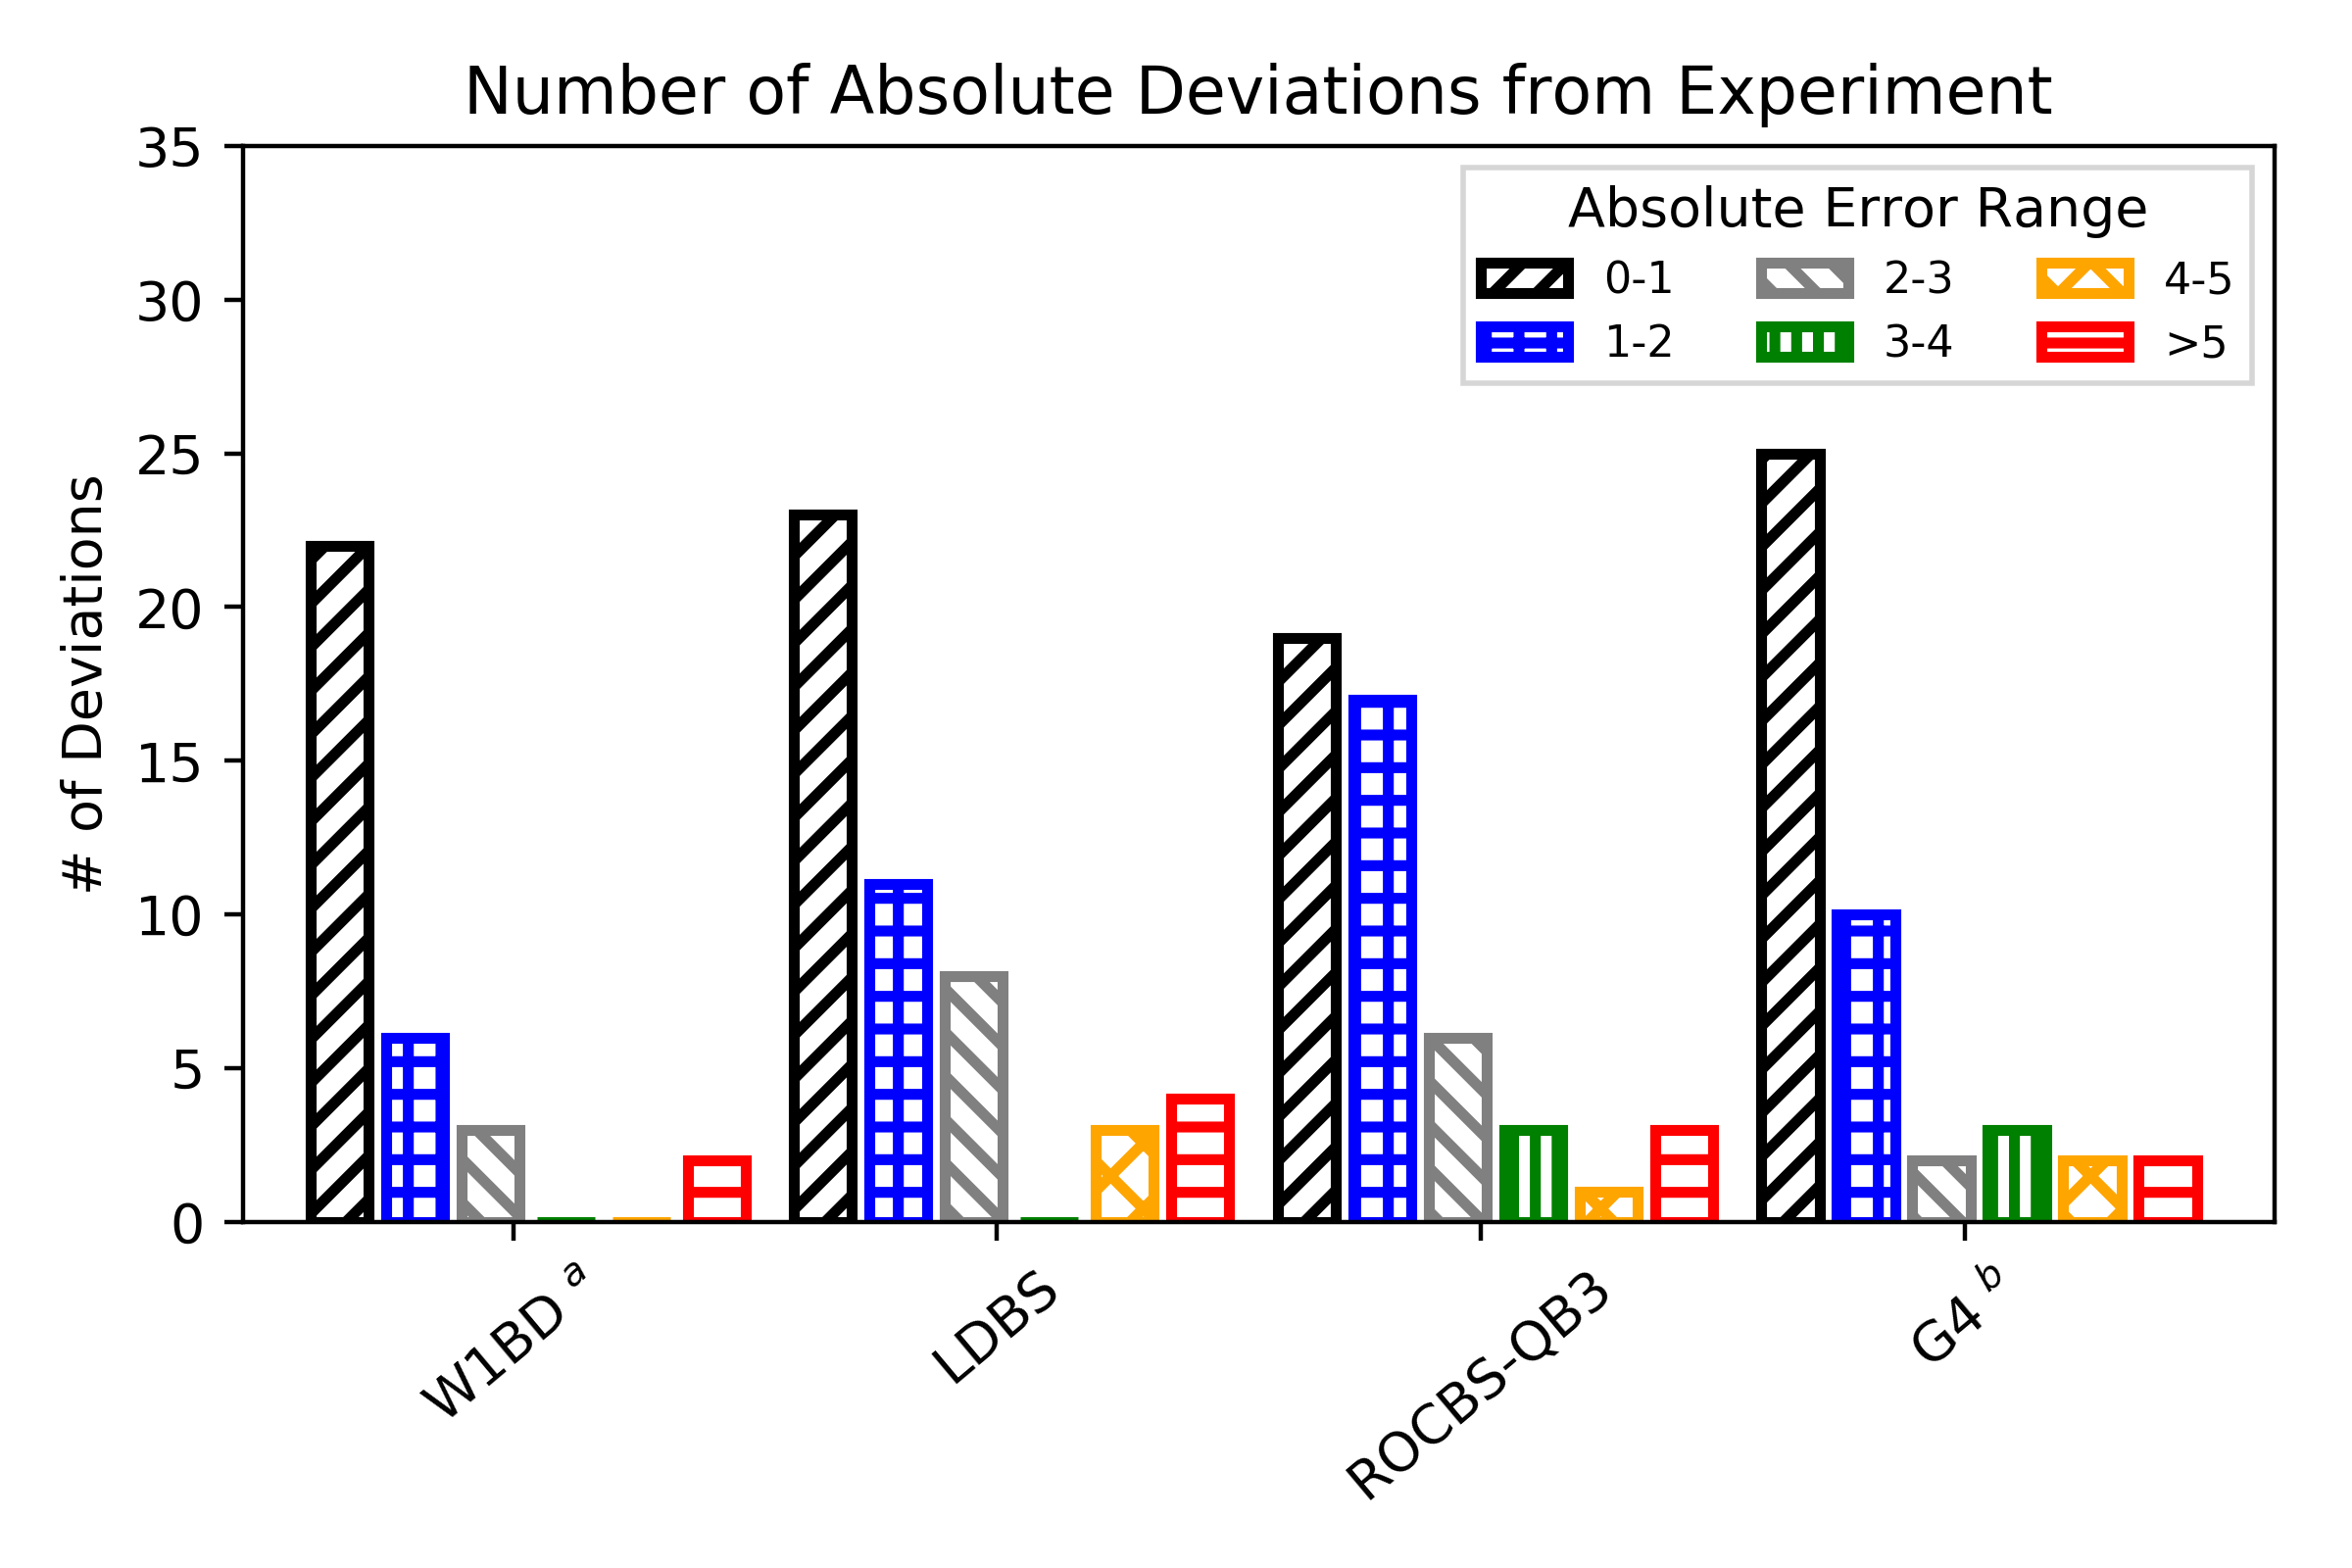
\includegraphics[width=\textwidth]{figures/bde-barchart}
  \caption[Summary of deviations of BDEs from literature for composite quantum chemical methods.]{Summary of deviations of BDEs from literature or composite quantum chemical methods. Errors are units of \kcalmol and are relative to Reference~\protect\citenum{Luo2002}. Numbers out of 49 represent the total number of data points which were computed for the given method.}
  \label{fig:maebarchart}
\end{figure}

Comparing W1BD results to literature, the MAE is 0.82 \kcalmol, with the majority of the data falls within 1--2 \kcalmol of each other. This suggests that W1BD is consistent with the literature values. There are, however, two large outliers: dimethylsulfoxide\footnotemark~ and \emph{N,N}-dimethylacetamide, with experiment underestimating the BDEs by -8.0 and -8.2 \kcalmol, respectively. This result is consistent amongst all composite method, verifying the inaccuracy of these results.

\footnotetext{The experimental BDE for dimethylsulfoxide was previously identified as accurate by Salamone et al.\protect\cite{Salamone2012}}

The best agreement with both W1BD and literature is the ROCBS-QB3 method (MAE = 0.18 (1.64) \kcalmol). In comparison, CBS-QB3 has an MAE = 0.32 (1.88) \kcalmol, while CBS-APNO has an MAE = 0.20 (1.40) \kcalmol.  The G4 method deviates from the W1BD reference by about 0.5 \kcalmol more, however, it appears to give reasonable agreement with experimental results (MAE = 0.70 (1.21) mol). The use of the MP2 variant of G4 gives somewhat questionable results, with an MAE of 0.88 (1.60) \kcalmol, as well as a large outlier of 6.2 kcal/mol that is not present in the other data from composite methods.

An alternative method for visualising these data is through the use of one-to-one plots, in which BDEs from two methods are directly compared. An ideal plot should have a slope = 1 and y-intercept = 0. These plots are reported in Appendix X, \jnote{FIG REF}, where it can once seen that ROCBS-QB3 performs best for the calculation of BDEs while G4(MP2) performs worst. Given these data, and considering the relative computational cost, the ROCBS-QB3 method is recommended for the efficient calculation of accurate BDEs, particularly for large molecules for which more expensive computational methods are not possible. Importantly, we can now confidently continue investigating the BEP relationships using reliable calculated BDE data from the ROCBS-QB3 method.

\section{Analysis of the Bell-Evans-Polanyi principle}

We turn now to the application of accurate BDEs on the BEP principle. Experimental HAT rate constants have been collected for 32 reactions involving \cumo and organic substrates. The BEP plot of the logarithm of normalised rate constants against BDEs is shown in~\ref{fig:bde-bep}.

There clearly exists two general trends in~\ref{fig:bde-bep}, inline with our initial hypothesis that there should exist two linear relations: one for benzylic/allylic C-H bonds and another for alkyl C-H bonds. However, the correlation of one of these trends is poor, a result which is inconsistent with our hypothesis. For the series of C-H BDEs which result in a radical which is delocalised, the correlation coefficient is 0.89, suggesting a valid correlation. Therefore, there is predictive power from a BEP relation for C-H bond cleavage which results in a delocalised radical. Furthermore, this result is consistent with the correlation of rate constants with C-H BDEs for model unsaturated fatty acids, described by Pratt et al.\cite{Pratt2003}

\begin{figure}[H]
  \centering
  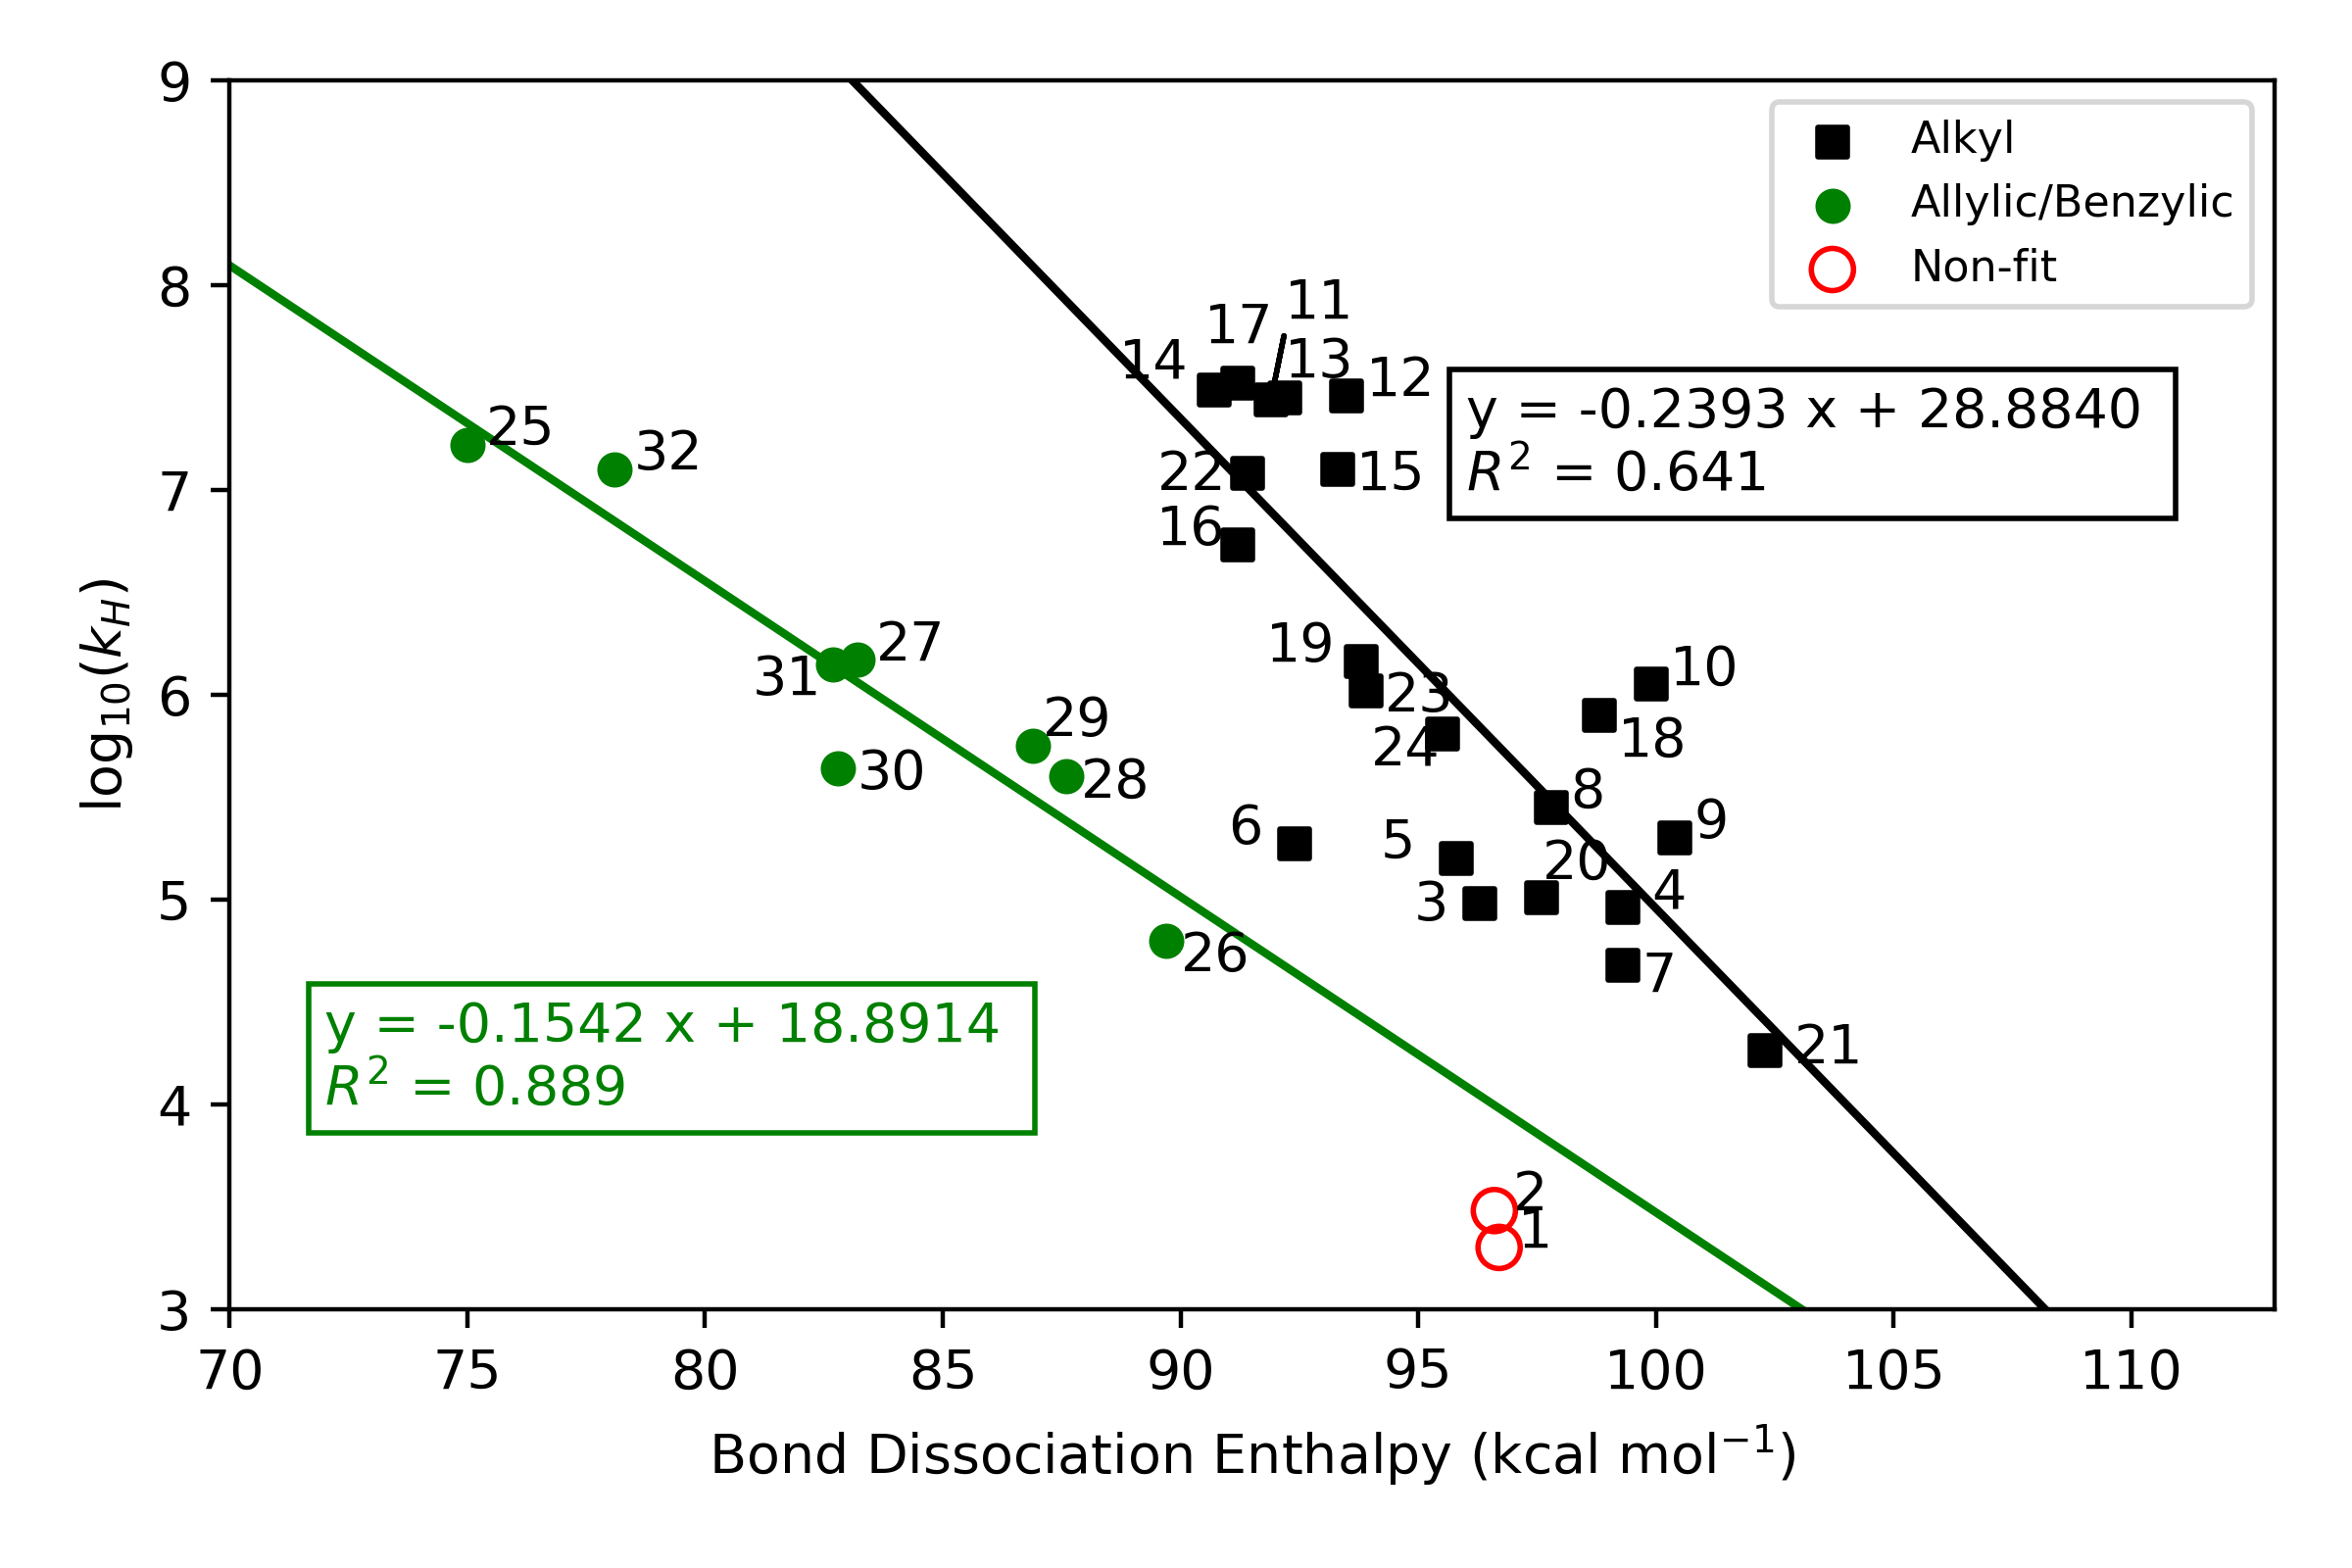
\includegraphics[width=\textwidth]{figures/bde-bep}
\begin{tabularx}{\textwidth}{| l X l X |}
  \hline
  1 & Acetone & 2 & Acetonitrile \\
  3 & Cyclopentane & 4 & 2,2-dimethylbutane \\
  5 & 2,3-dimethylbutane & 6 & Cyclohexane \\
  7 & Cycloheptane & 8 & Cyclooctane \\
  9 & Adamantane (2$^\circ$) & 10 & Adamantane (3$^\circ$) \\
  11 & Diethyl Ether & 12 & Piperazine \\
  13 & Piperidine & 14 & Pyrrolidine \\
  15 & Tetrahydrofuran & 16 & Dioxane \\
  17 & Triethylamine & 18 & DABCO \\
  19 & Dimethylsulfoxide & 20 & Benzaldehyde \\
  21 & HMPA & 22 & Morpholine \\
  23 & Diethylamine & 24 & Propylamine \\
  25 & Cyclohexadiene & 26 & Toluene \\
  27 & Benzyl Alcohol & 28 & Ethylbenzene \\
  29 & Cumene & 30 & Diphenylmethane \\
  31 & Dibenzyl Ether & 32 & 9,10-dihydroanthracene \\
  \hline
\end{tabularx}
  \caption{Bell-Evans-Polanyi plot of experimental rate constants for HAT between \cumo~ and substrates. Acetone and acetonitrile are note included in fitting as the experimental rate constants are approximate. Needs revision to move labels around.}
\label{fig:bde-bep}
\end{figure}

In contrast, the alkyl C-H BDEs shows very weak correlation with HAT rate constants, with a correlation coefficient of 0.63. However, with the exception of two larger outlier, cyclooctane and the secondary hydrogen position of adamantane, the majority of the data fall within half an order of magnitude of rate a rate constant which is consistent with the line of best fit. The two large outliers are approximately twice as far from the trendline. While this result may not seem positive, there is actually some predictive power in the BEP relation established for alkyl C-H bonds. This is because in the calculations of rate constants, an error of only 1.2 \kcalmol can result in a order of magnitude difference in rate constant. Errors of this magnitude are not uncommon for DFT-based mechanistic studies. For example, barrier heights for a set\cite{Zhao2005, Zhao2009} of 76 hydrogen transfer, heavy atom transfer, nucleophilic substitution, unimolecular, and association reactions calculated with at the B3LYP-D3(BJ)/Def2-QZVP level of theory give a mean absolute error of 5.20 \kcalmol, with errors exceeding 11 \kcalmol.\cite{Goerigk2011}

In sum, these results suggest that the BEP principle is overly simple to directly correlate the large groups of allylic/benzylic and alkyl C-H bonds with HAT rate constant. Nonetheless, BEP relations offer predictive capabilities for rate constants to within an order of magnitude. Importantly, this result indicates that there are additional factors which contribute to the HAT rate constants studied herein.

\section{Transition state analysis}

In order to determine what effects appear to be most important, I have calculated TS structures for 19 of the reactions at the LC-$\omega$PBE-D3(BJ)/6-311+G(2d,2p)//B3LYP-D3(BJ)/6-31+G$^*$ level of theory. Comparing the calculated rate constants both with and without tunnelling corrections, there is a large degree of variability in the agreement with experiment. \ref{fig:kH-theory} demonstrates that the calculated rate constants deviate rather significantly from the experimental rate constants, both with and without the inclusion of a tunnelling correction. This result is perhaps unsurprising given the neglect of solvent effects, and the fairly low level of theory used for optimisation. Note however, that the goal of these calculations was not to reproduce experimental rate constants, but to obtain TS complex structures to analyse the structural differences that may lead to the deviations from the BEP principle.

\begin{figure}[htb]
\centering
\begin{minipage}{8cm}
  \centering
  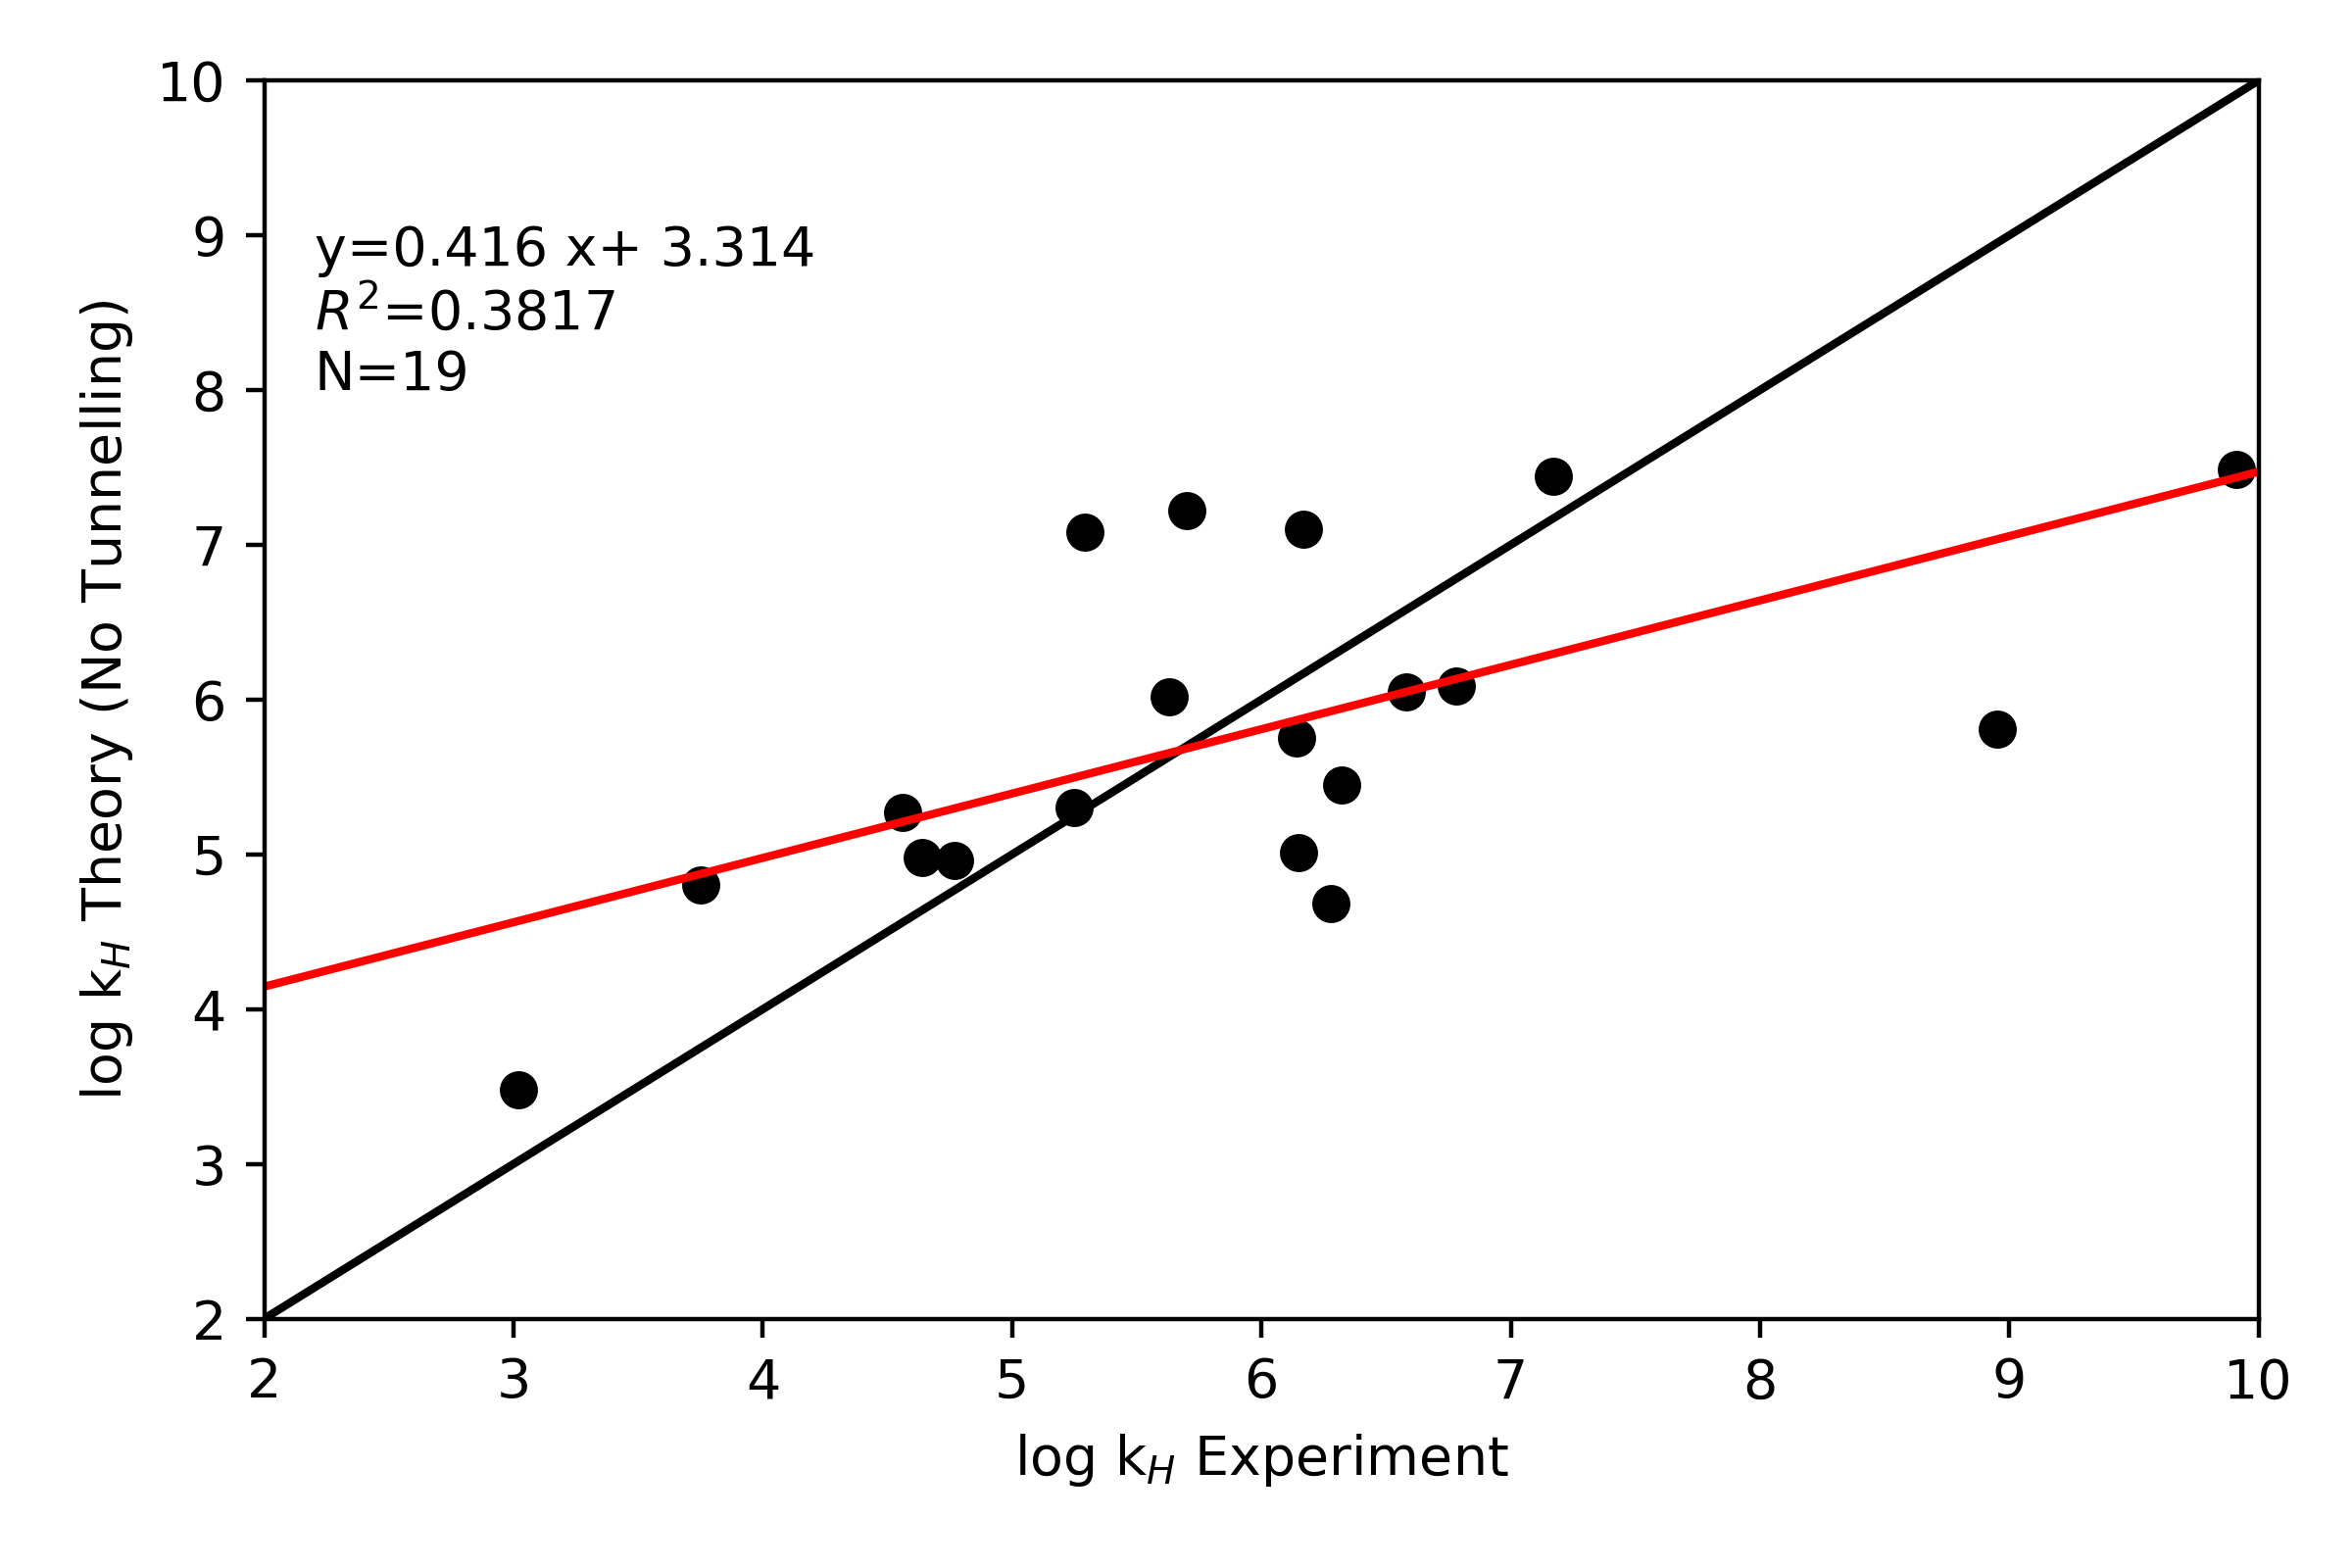
\includegraphics[width=\textwidth]{figures/kH-theorya}
\end{minipage}%
\begin{minipage}{8cm}
  \centering
  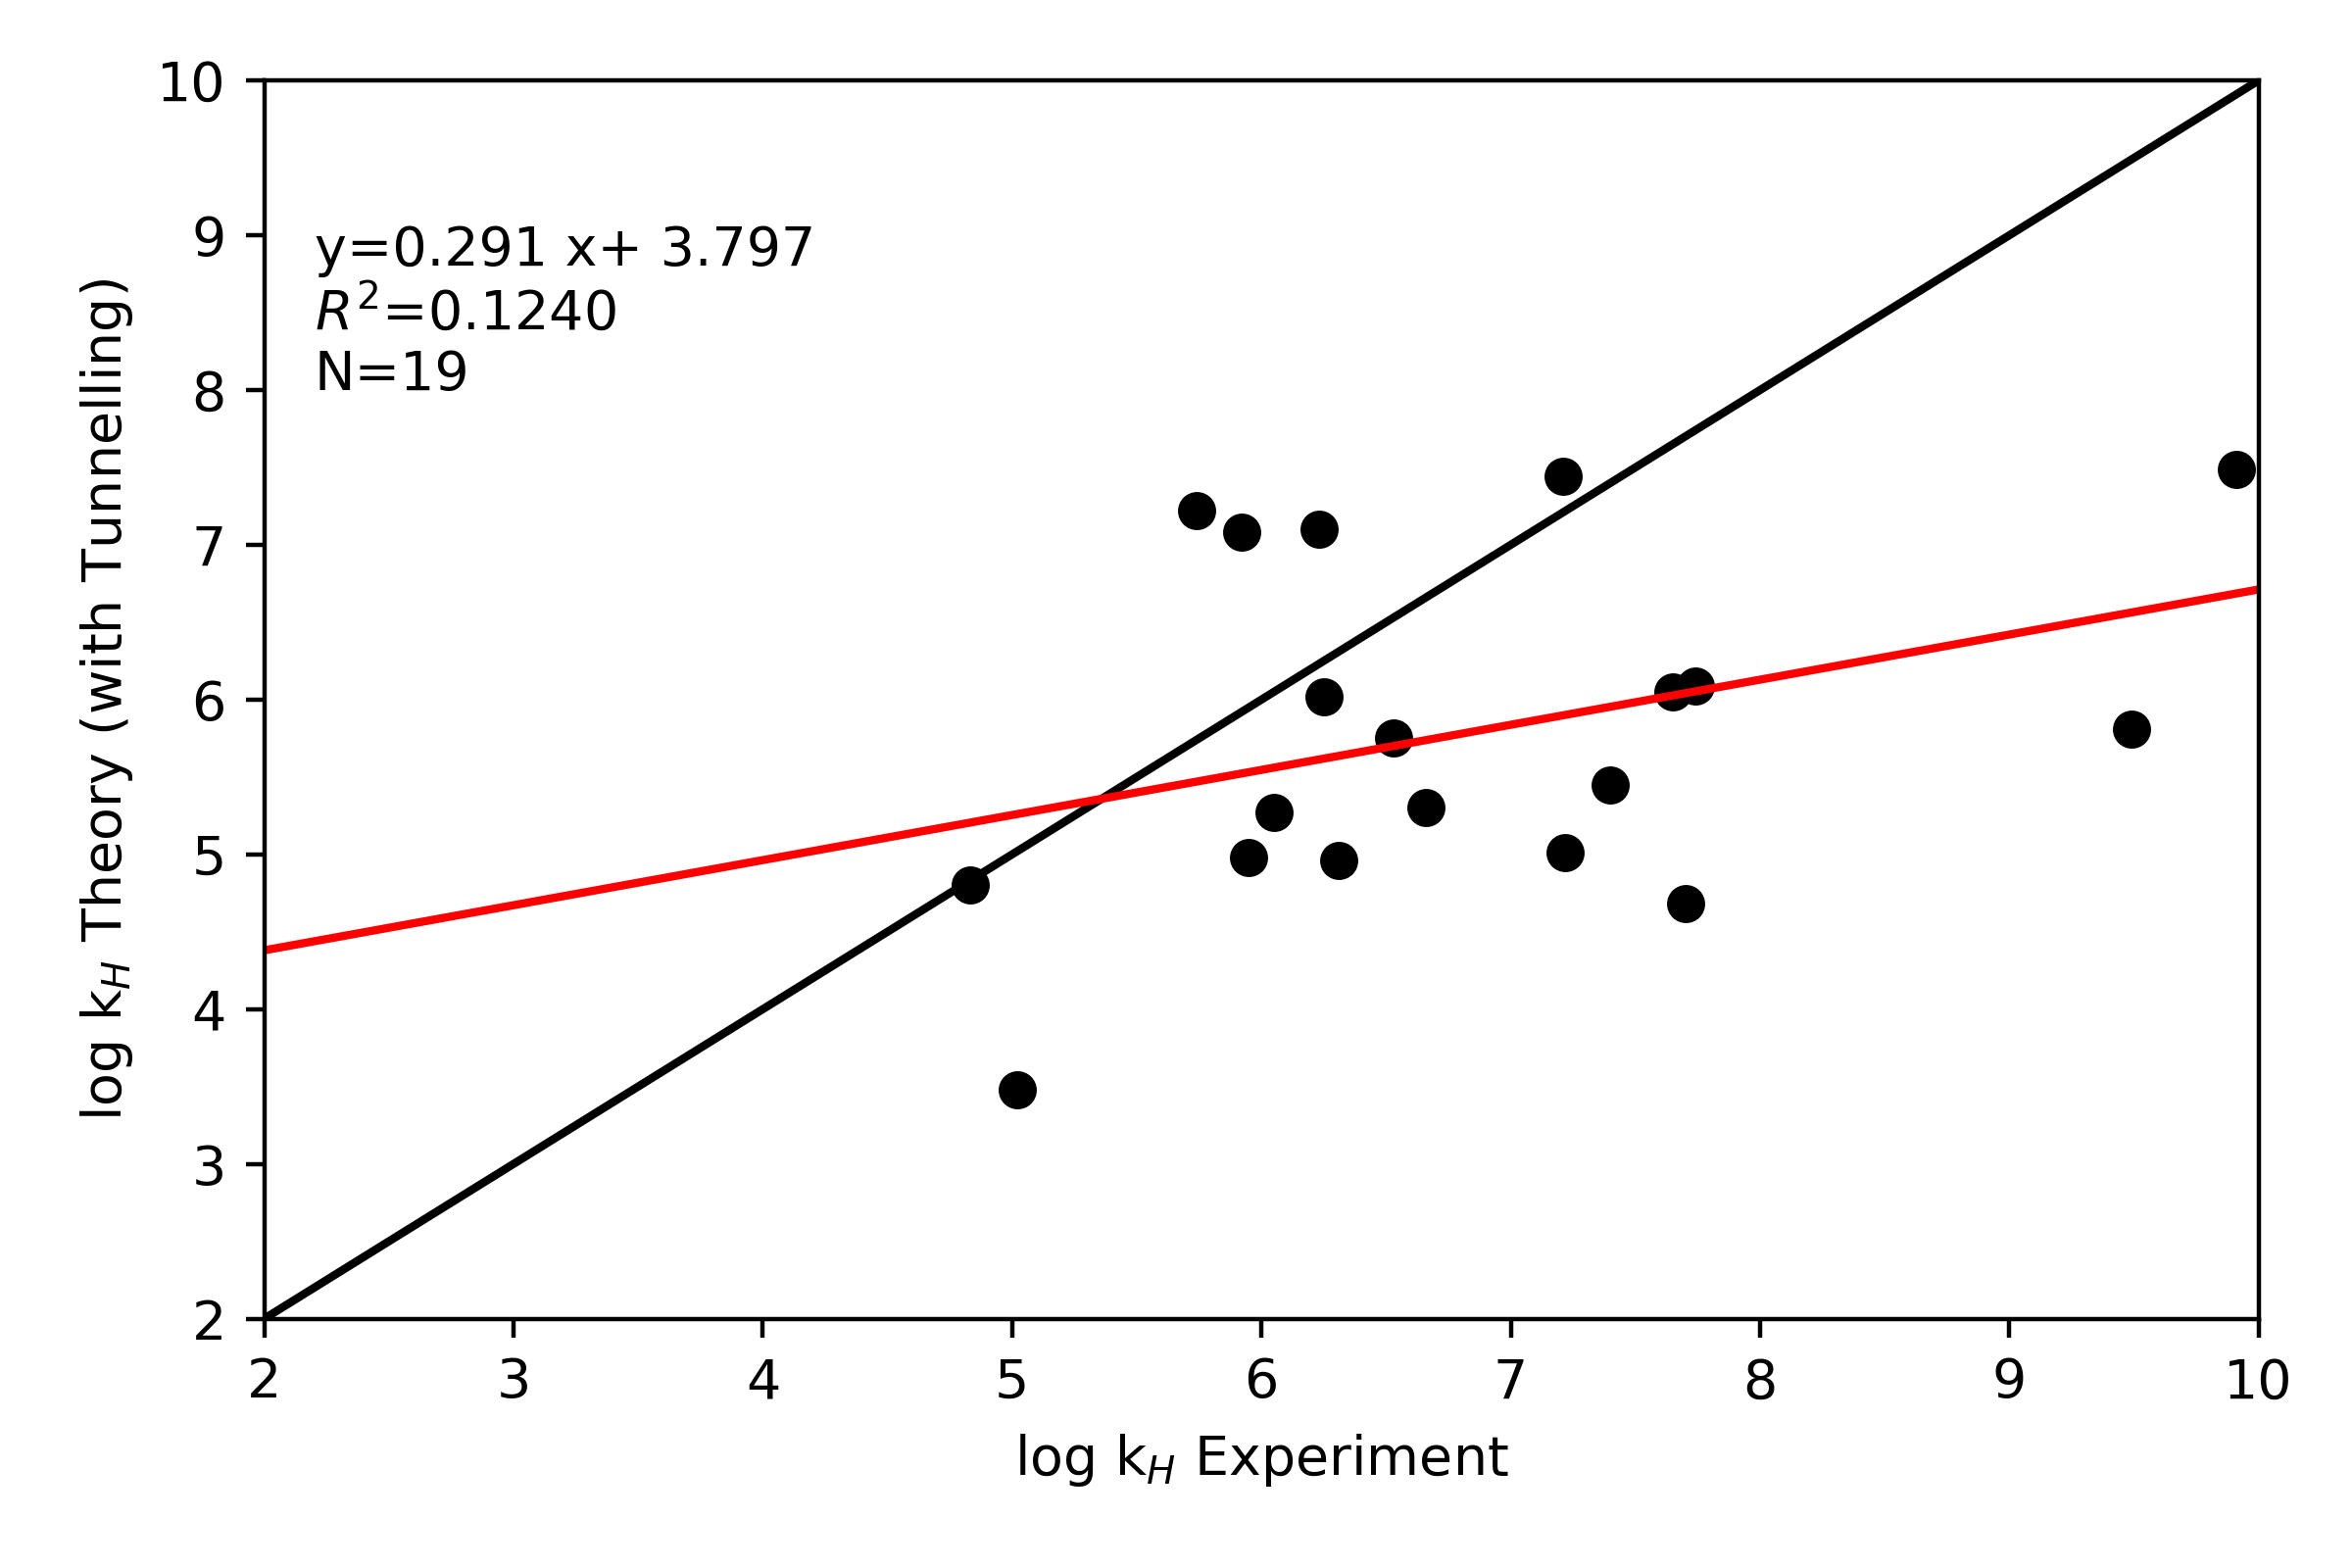
\includegraphics[width=\textwidth]{figures/kH-theoryb}
\end{minipage}
\caption[One-to-one plots of theoretically determined logarithm of rate constant or HAT reactions between \cumo~ and organic substrates against experimental values.]{One-to-one plots of theoretically determined logarithm of rate constant for HAT reactions between \cumo~ and organic substrates against experimental values. The plot on the left does not include a tunnelling correction while the plot on the right includes the Eckart potential tunnelling correction.}
\label{fig:kH-theory}
\end{figure}

The first factor which may lead to deviations from the BEP is the possibility for different HAT reaction mechanisms, i.e. direct HAT or PCET. Consider first the reaction of toluene with \cumo. As this reaction is similar to the self-exchange reaction of the benzyl-toluene couple as described by DiLabio and Johnson,\cite{DiLabio2007} one might expect the reaction to proceed via PCET. The lowest energy TS complex has a partially $\pi$-stacked conformation with the rings oriented about 40$^\circ$ relative to one another. Surprisingly, examination of the SOMO and HOMO reveals no $\pi$-$\pi$ partial bonding interaction, as can be seen in~\ref{fig:cumo-toluene}. The electron density of the SOMO is largely localised on the toluene portion of the complex. This is likely due to the additional non-conjugated carbon centre of \cumo, which prevent an additional electron channel for PCET to occur. Therefore, this reaction takes place through direct HAT. This behaviour is specific to the \cumo radical, thus all the reactions likely also take place through a direct HAT mechanism, and this should not factor into the deviations in the observed BEP principle relationships.

\begin{figure}[htb]
  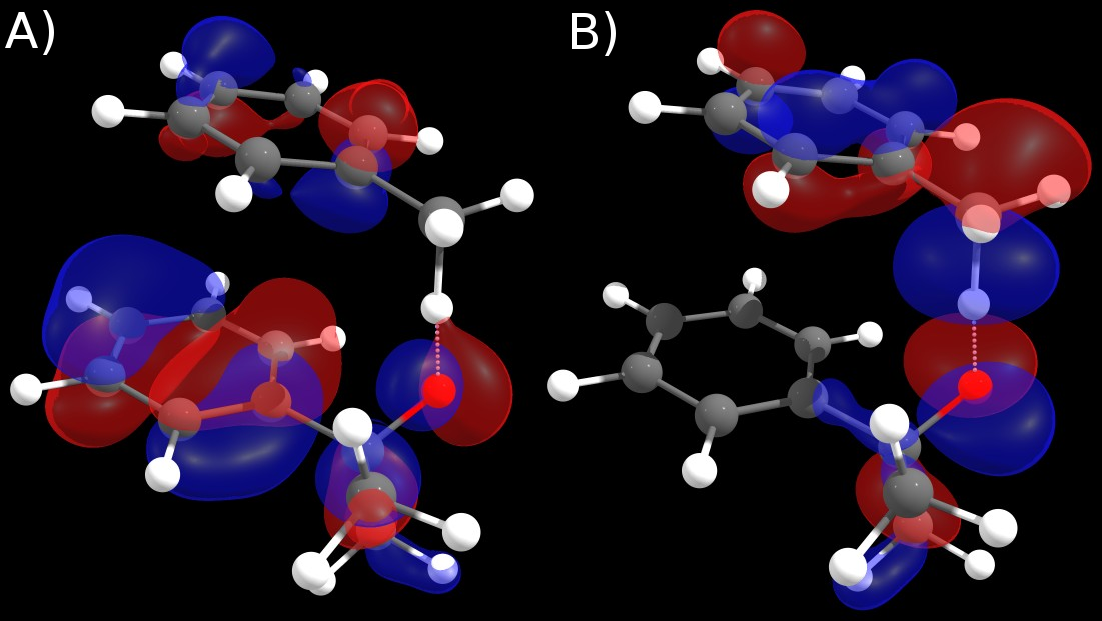
\includegraphics[width=\textwidth]{figures/cumo-toluene}
  \caption{Insert better images of \cumo-toluene TS complex with A) SOMO and B) HOMO.}
  \label{fig:cumo-toluene}
\end{figure}

There are several other possible deviations which may arise from differences in intermolecular interactions due to structural differences in the substrates. For example, cyclooctane may deviate from the trend observed due to the many possible conformations of the ring which are comparable in energy.\cite{Dorofeeva1985} Alternatively, the position of the TS complex along the reaction coordinate may differ between the various reactions. This would break the assumption of the BEP principle, and may result in deviation from the expected trend.

\jnote{I am having a hard time finding further explanations from the data I have. Any input here is greatly appreciated.}

\section{Summary}

Firstly, a number of composite quantum mechanical methods were tested for the accurate prediction of C-H BDEs. The ROCBS-QB3 method was determined to be the most efficient accurate method for this purpose. Additionally, the widespread applicability of the BEP principle was investigated through utilisation of these accurate C-H BDEs and experimental HAT rate constants for reaction of \cumo with organic substrates.

As was hypothesised, two relationships exist for the BEP principle when investigating a wide range of HAT reactions from C-H bonds. C-H bonds which result in a radical which can be delocalised into neighbour $\pi$ systems (benzylic/allylic) correlate well with experimental rate constants. The remaining alkyl C-H bonds, correlate weakly with experimental rate constants and offer only order of magnitude predictions of rate constants. Altogether, these results suggest that the BEP principle must be carefully applied if accurate rate constants are the desired target, however, they also suggest that as the BEP principle holds as a reasonably general principle.

\newpage
\section{Data and figures to be moved to appendix}

\begin{figure}
  \centering
  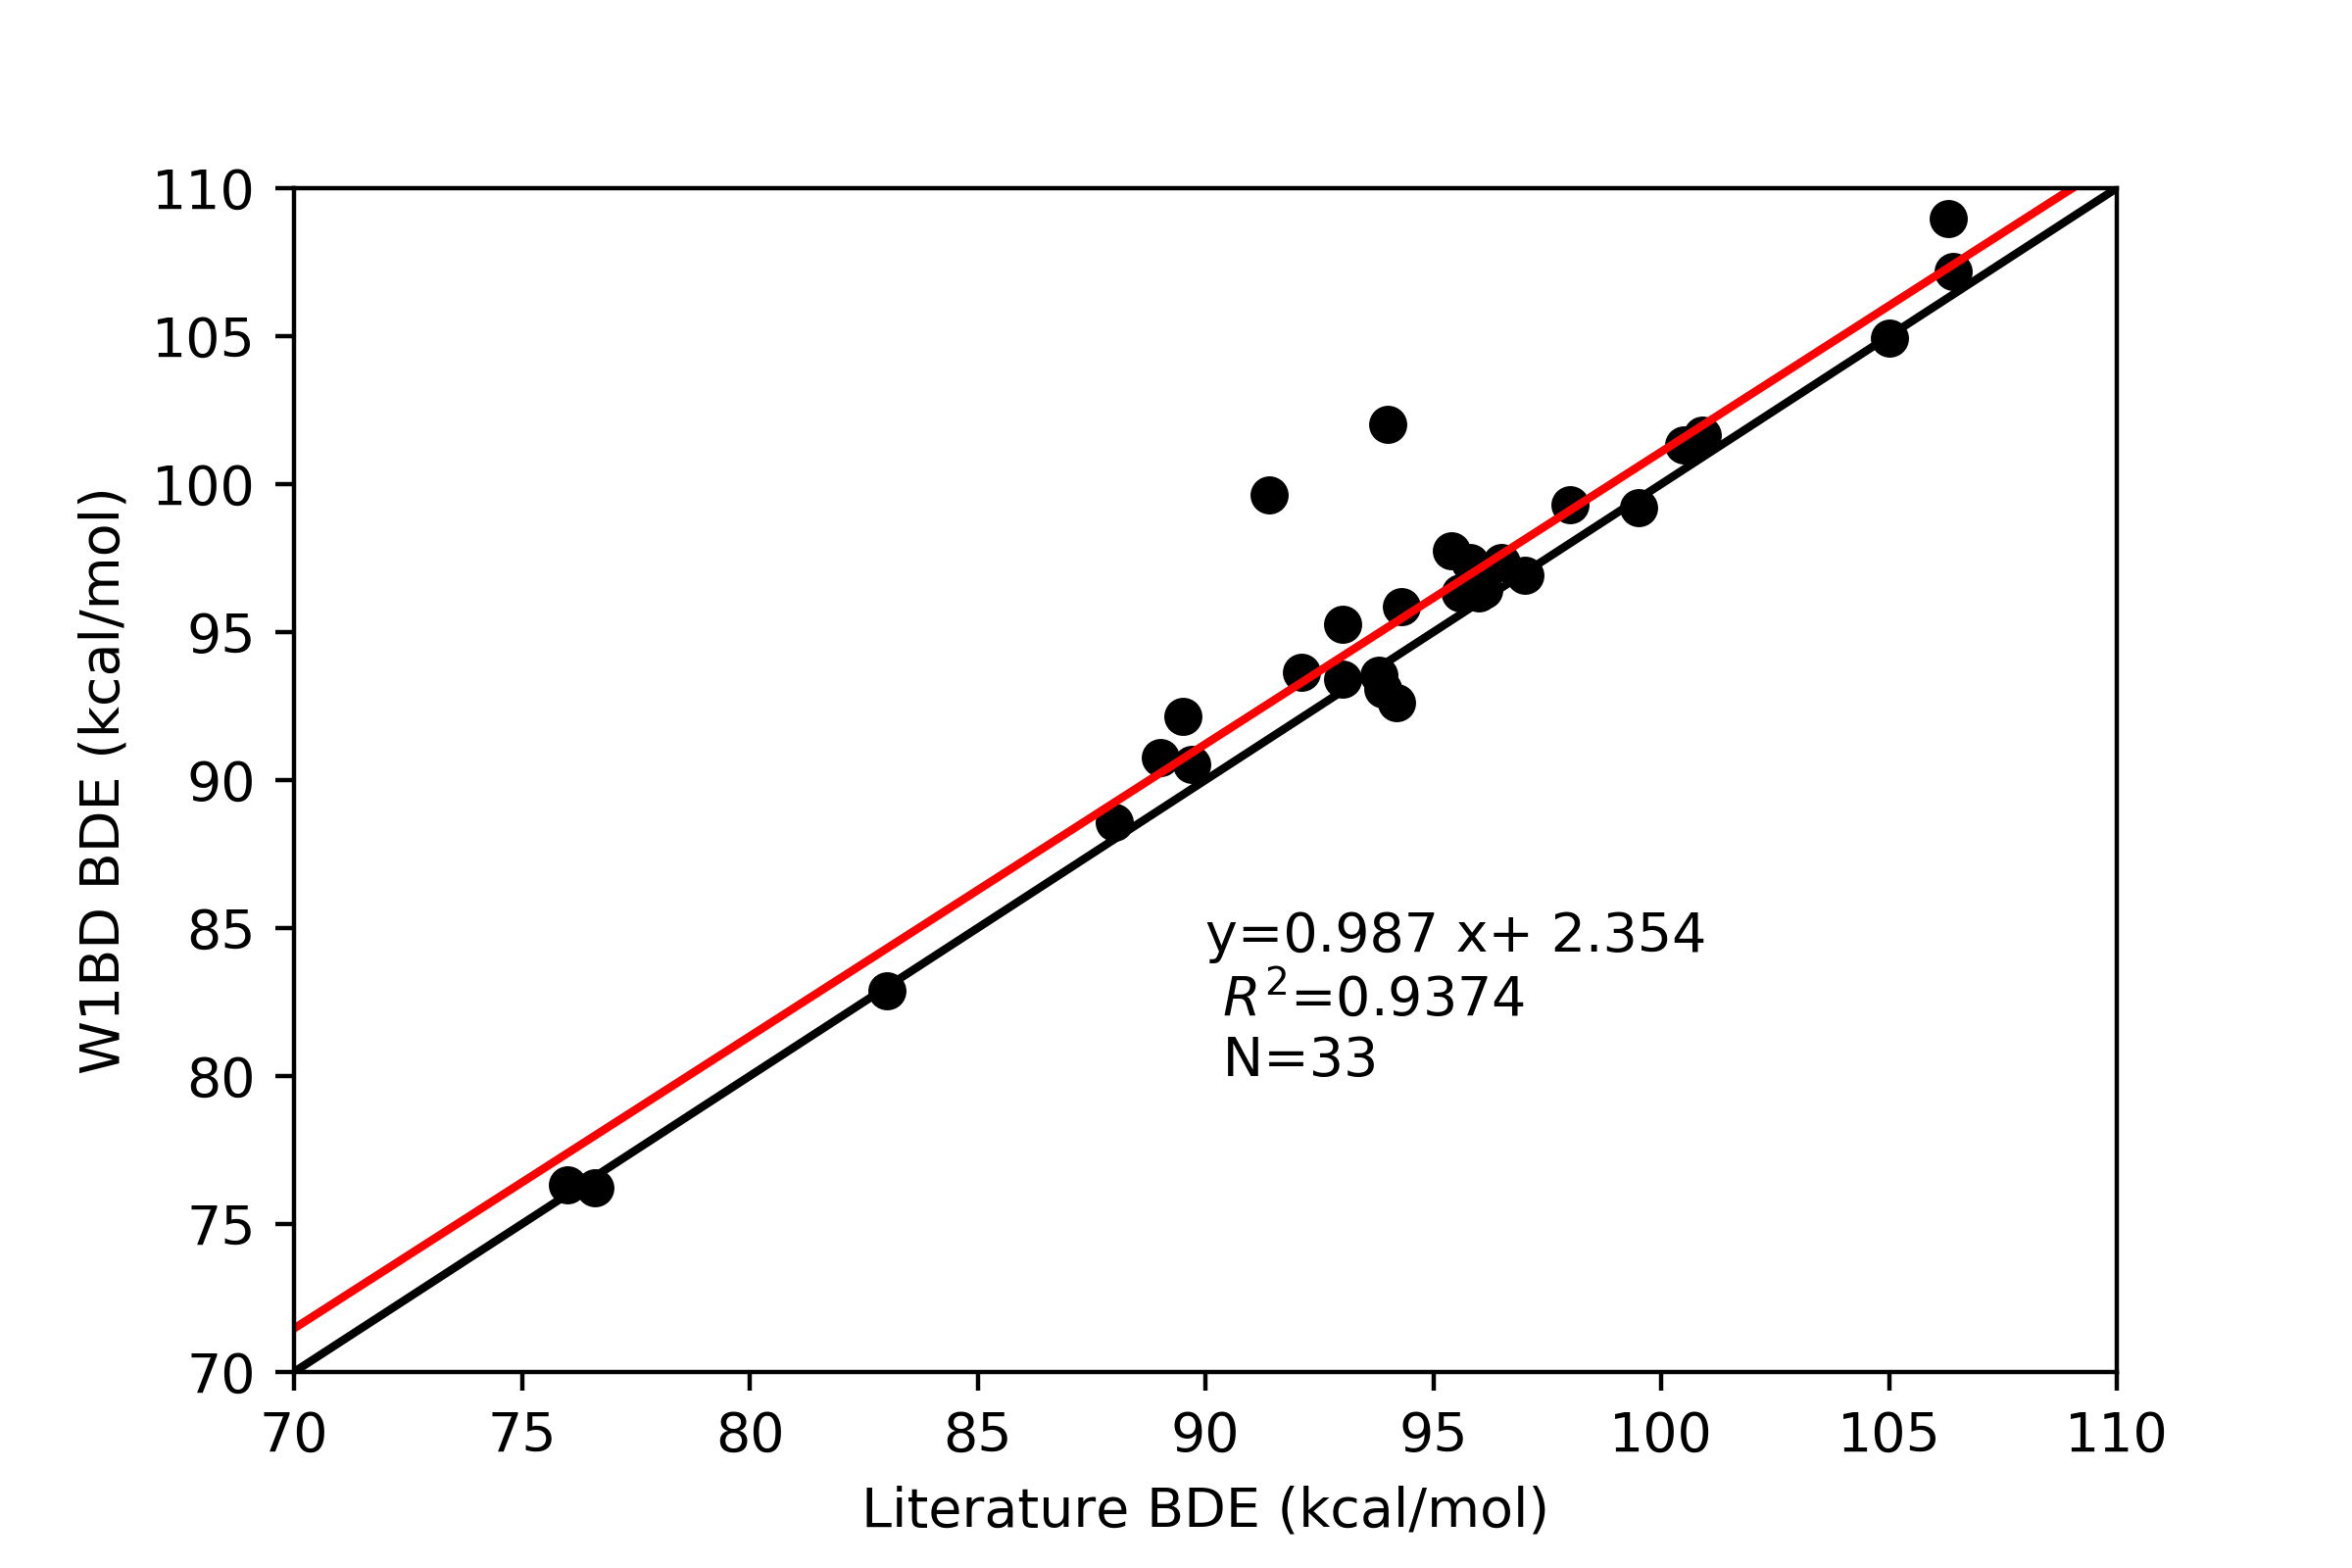
\includegraphics[width=0.7\textwidth]{figures/lit-w1bd}
\end{figure}


\begin{figure}
\centering
\begin{minipage}{8cm}
  \centering
  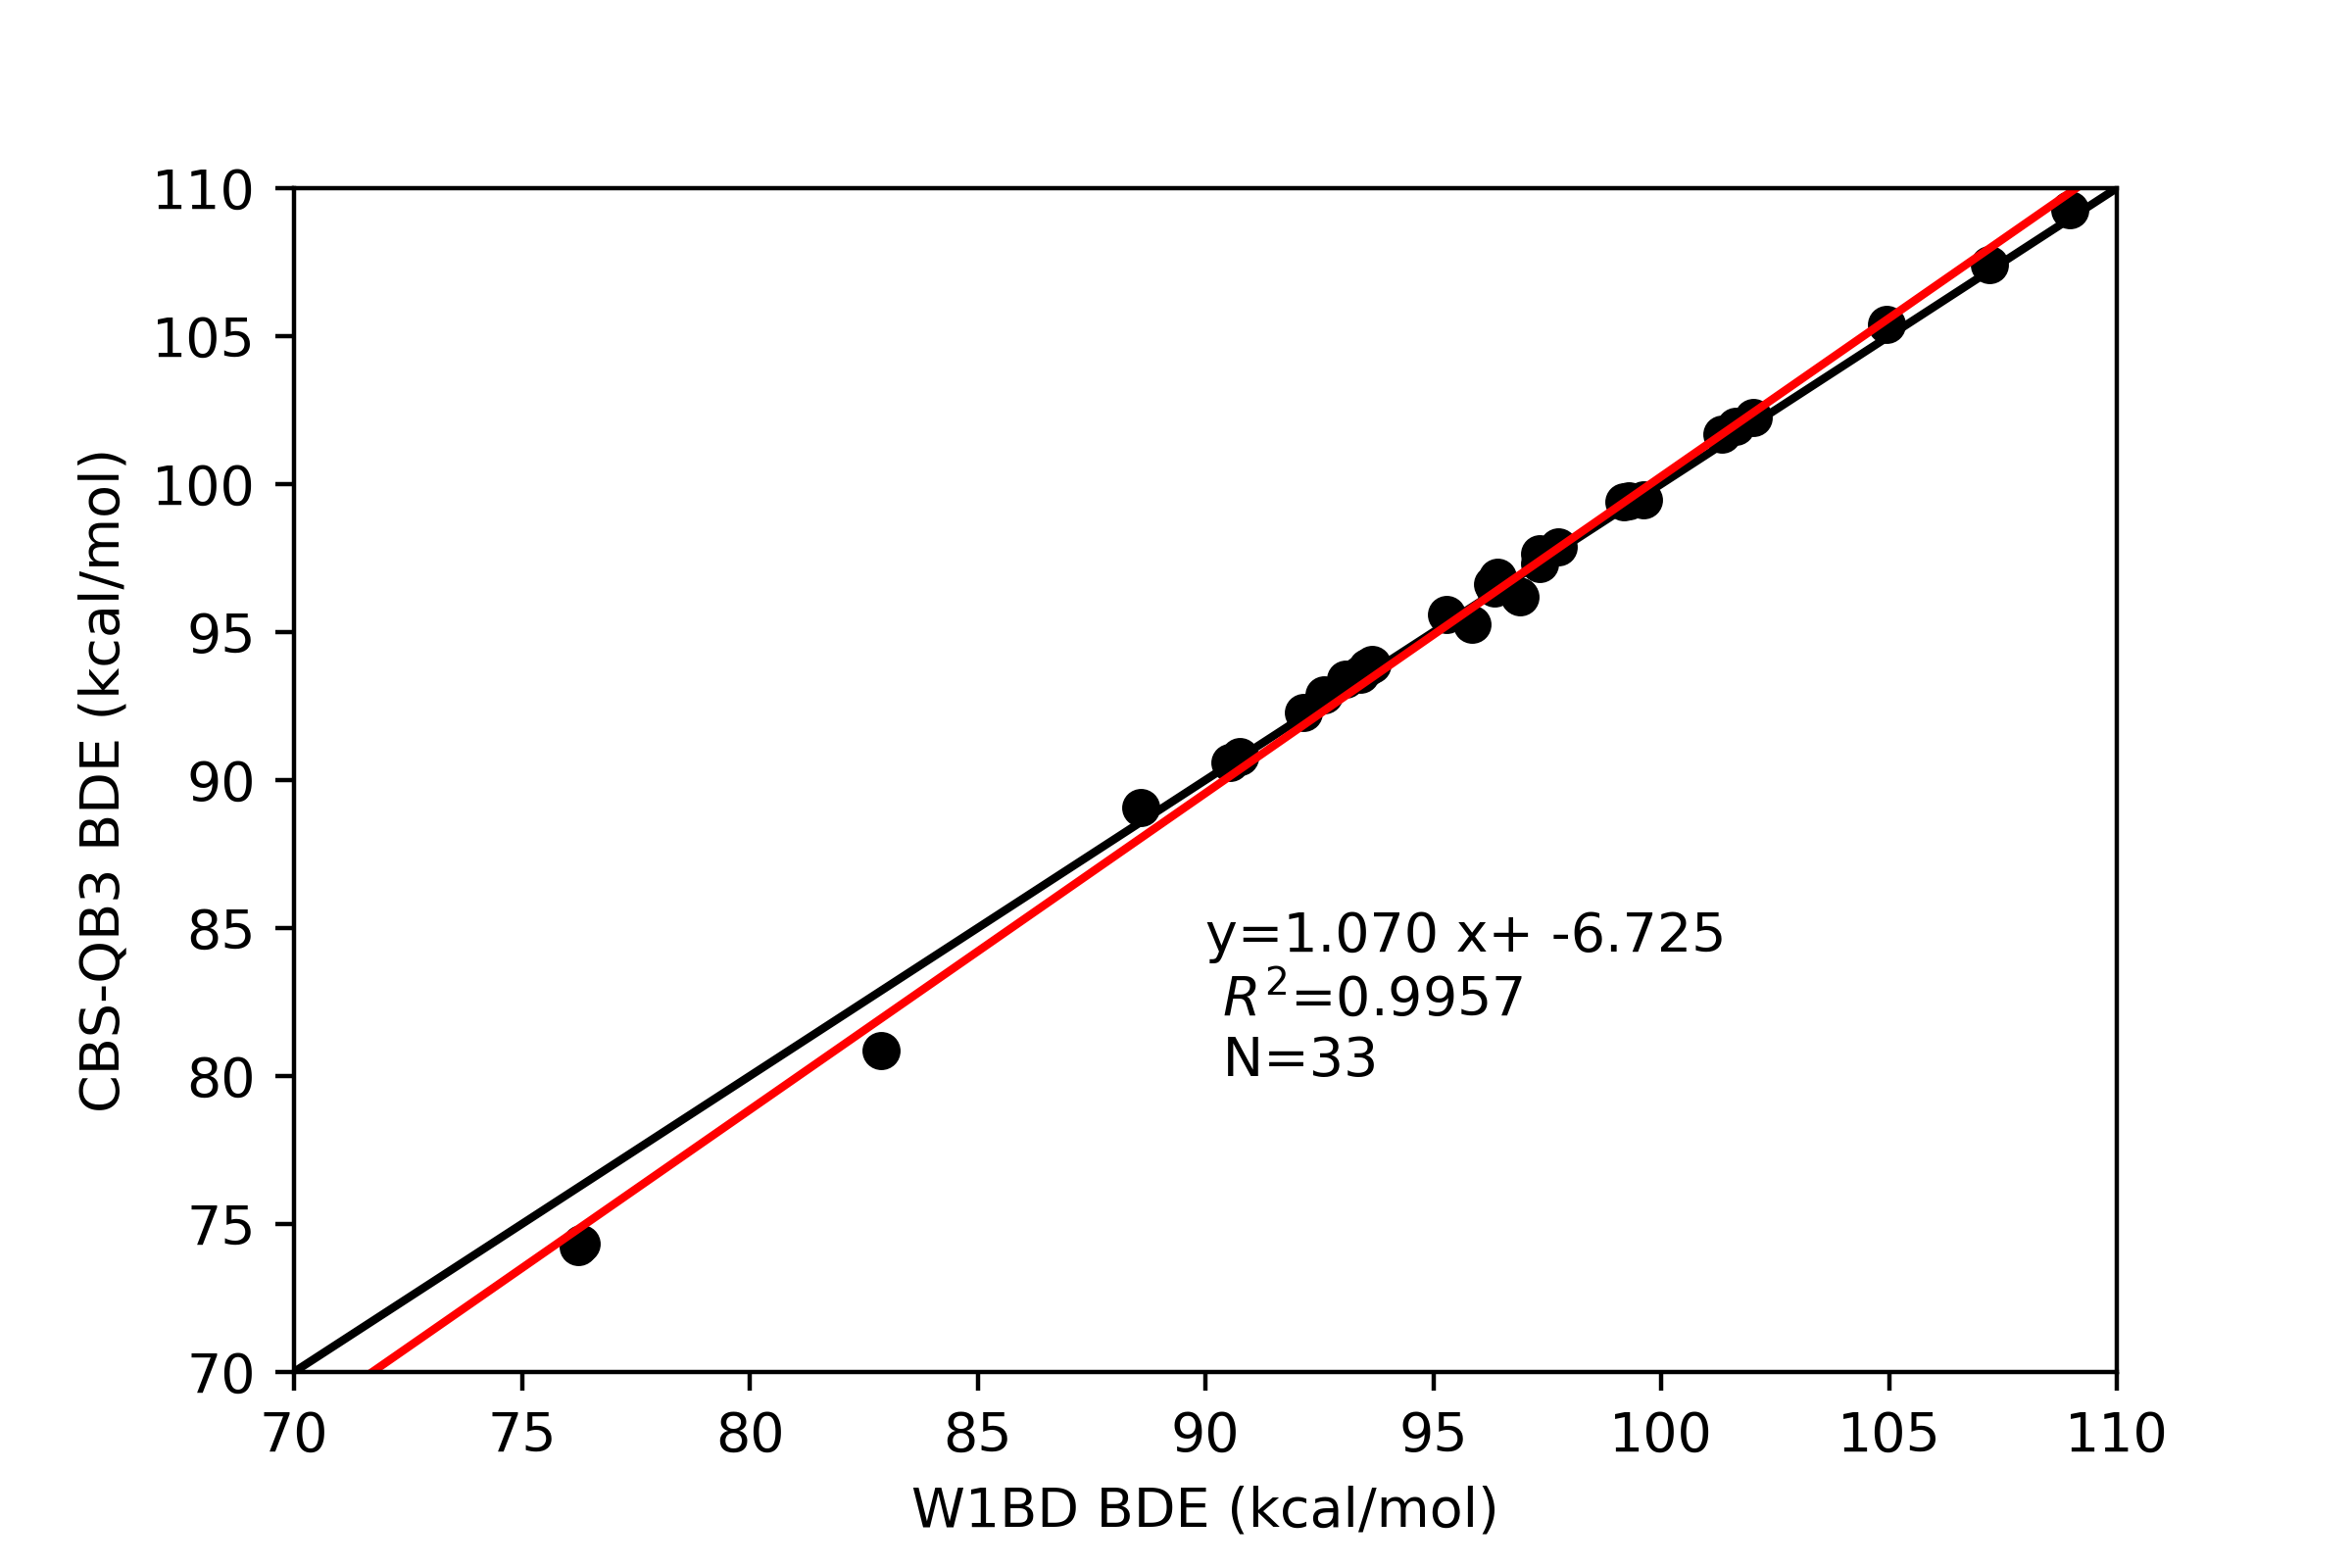
\includegraphics[width=\textwidth]{figures/w1bd-cbsqb3}
\end{minipage}%
\begin{minipage}{8cm}
  \centering
  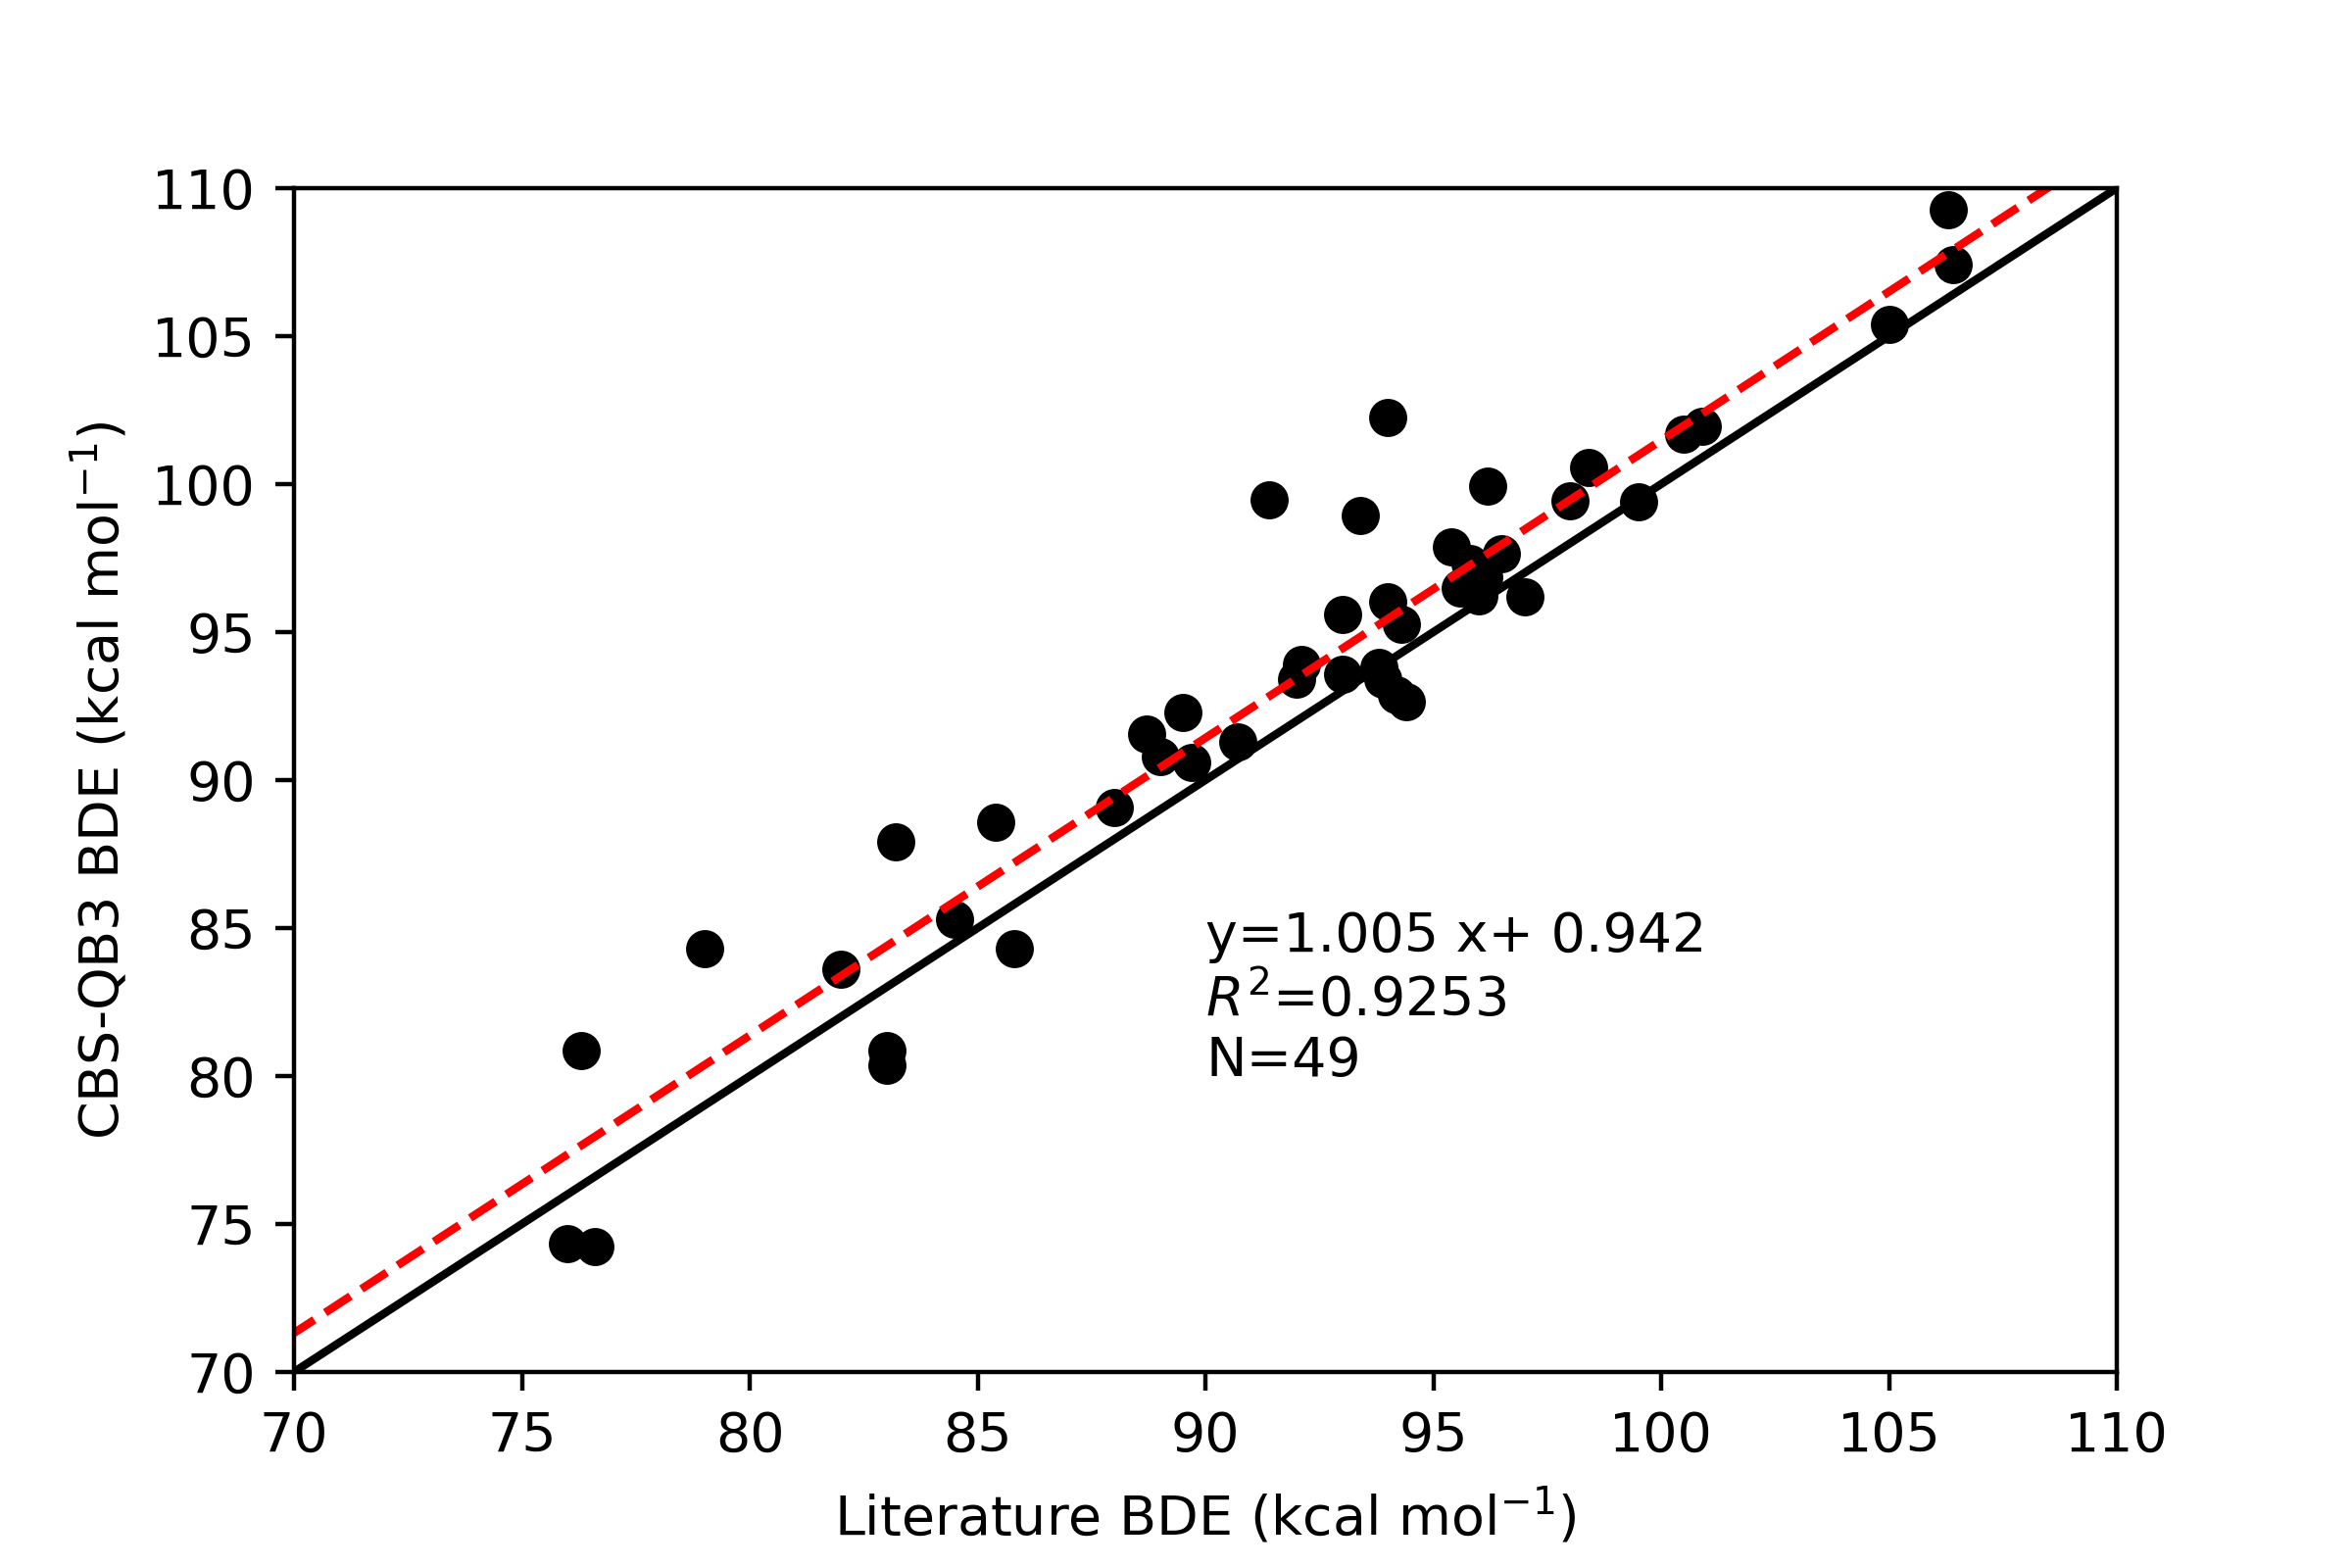
\includegraphics[width=\textwidth]{figures/lit-cbsqb3}
\end{minipage}
\end{figure}

\begin{figure}
\centering
\begin{minipage}{8cm}
  \centering
  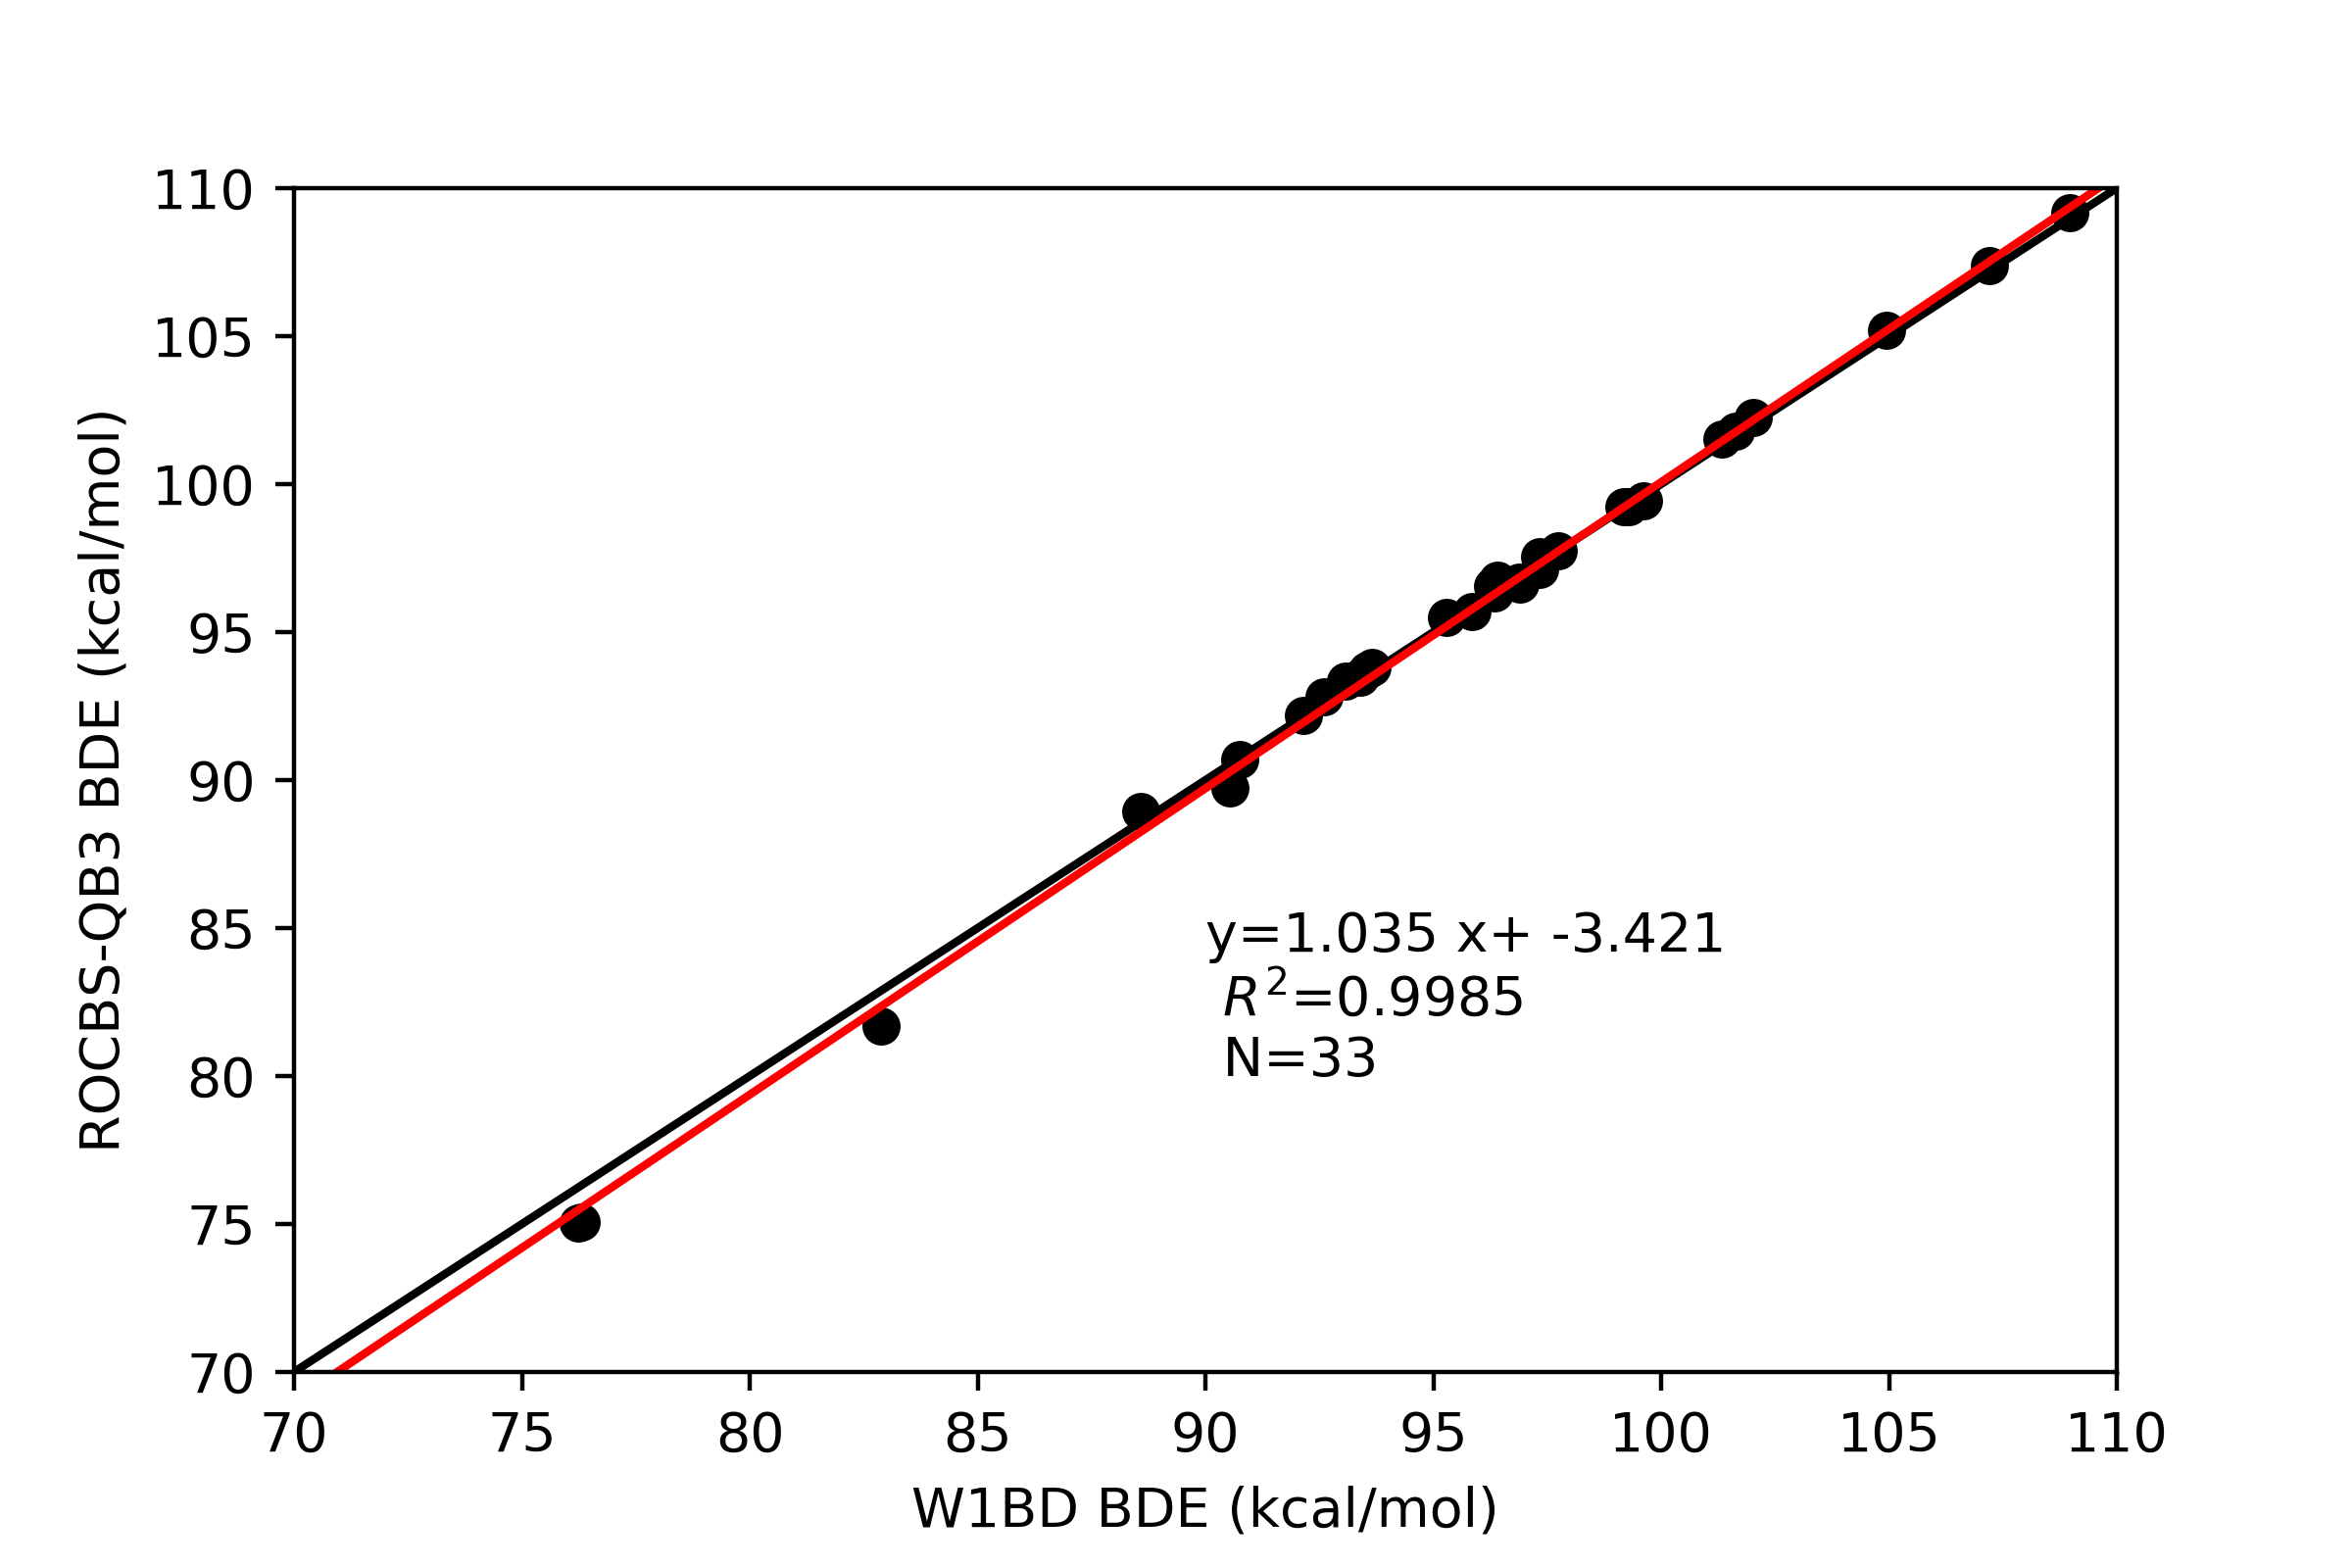
\includegraphics[width=\textwidth]{figures/w1bd-rocbsqb3}
\end{minipage}%
\begin{minipage}{8cm}
  \centering
  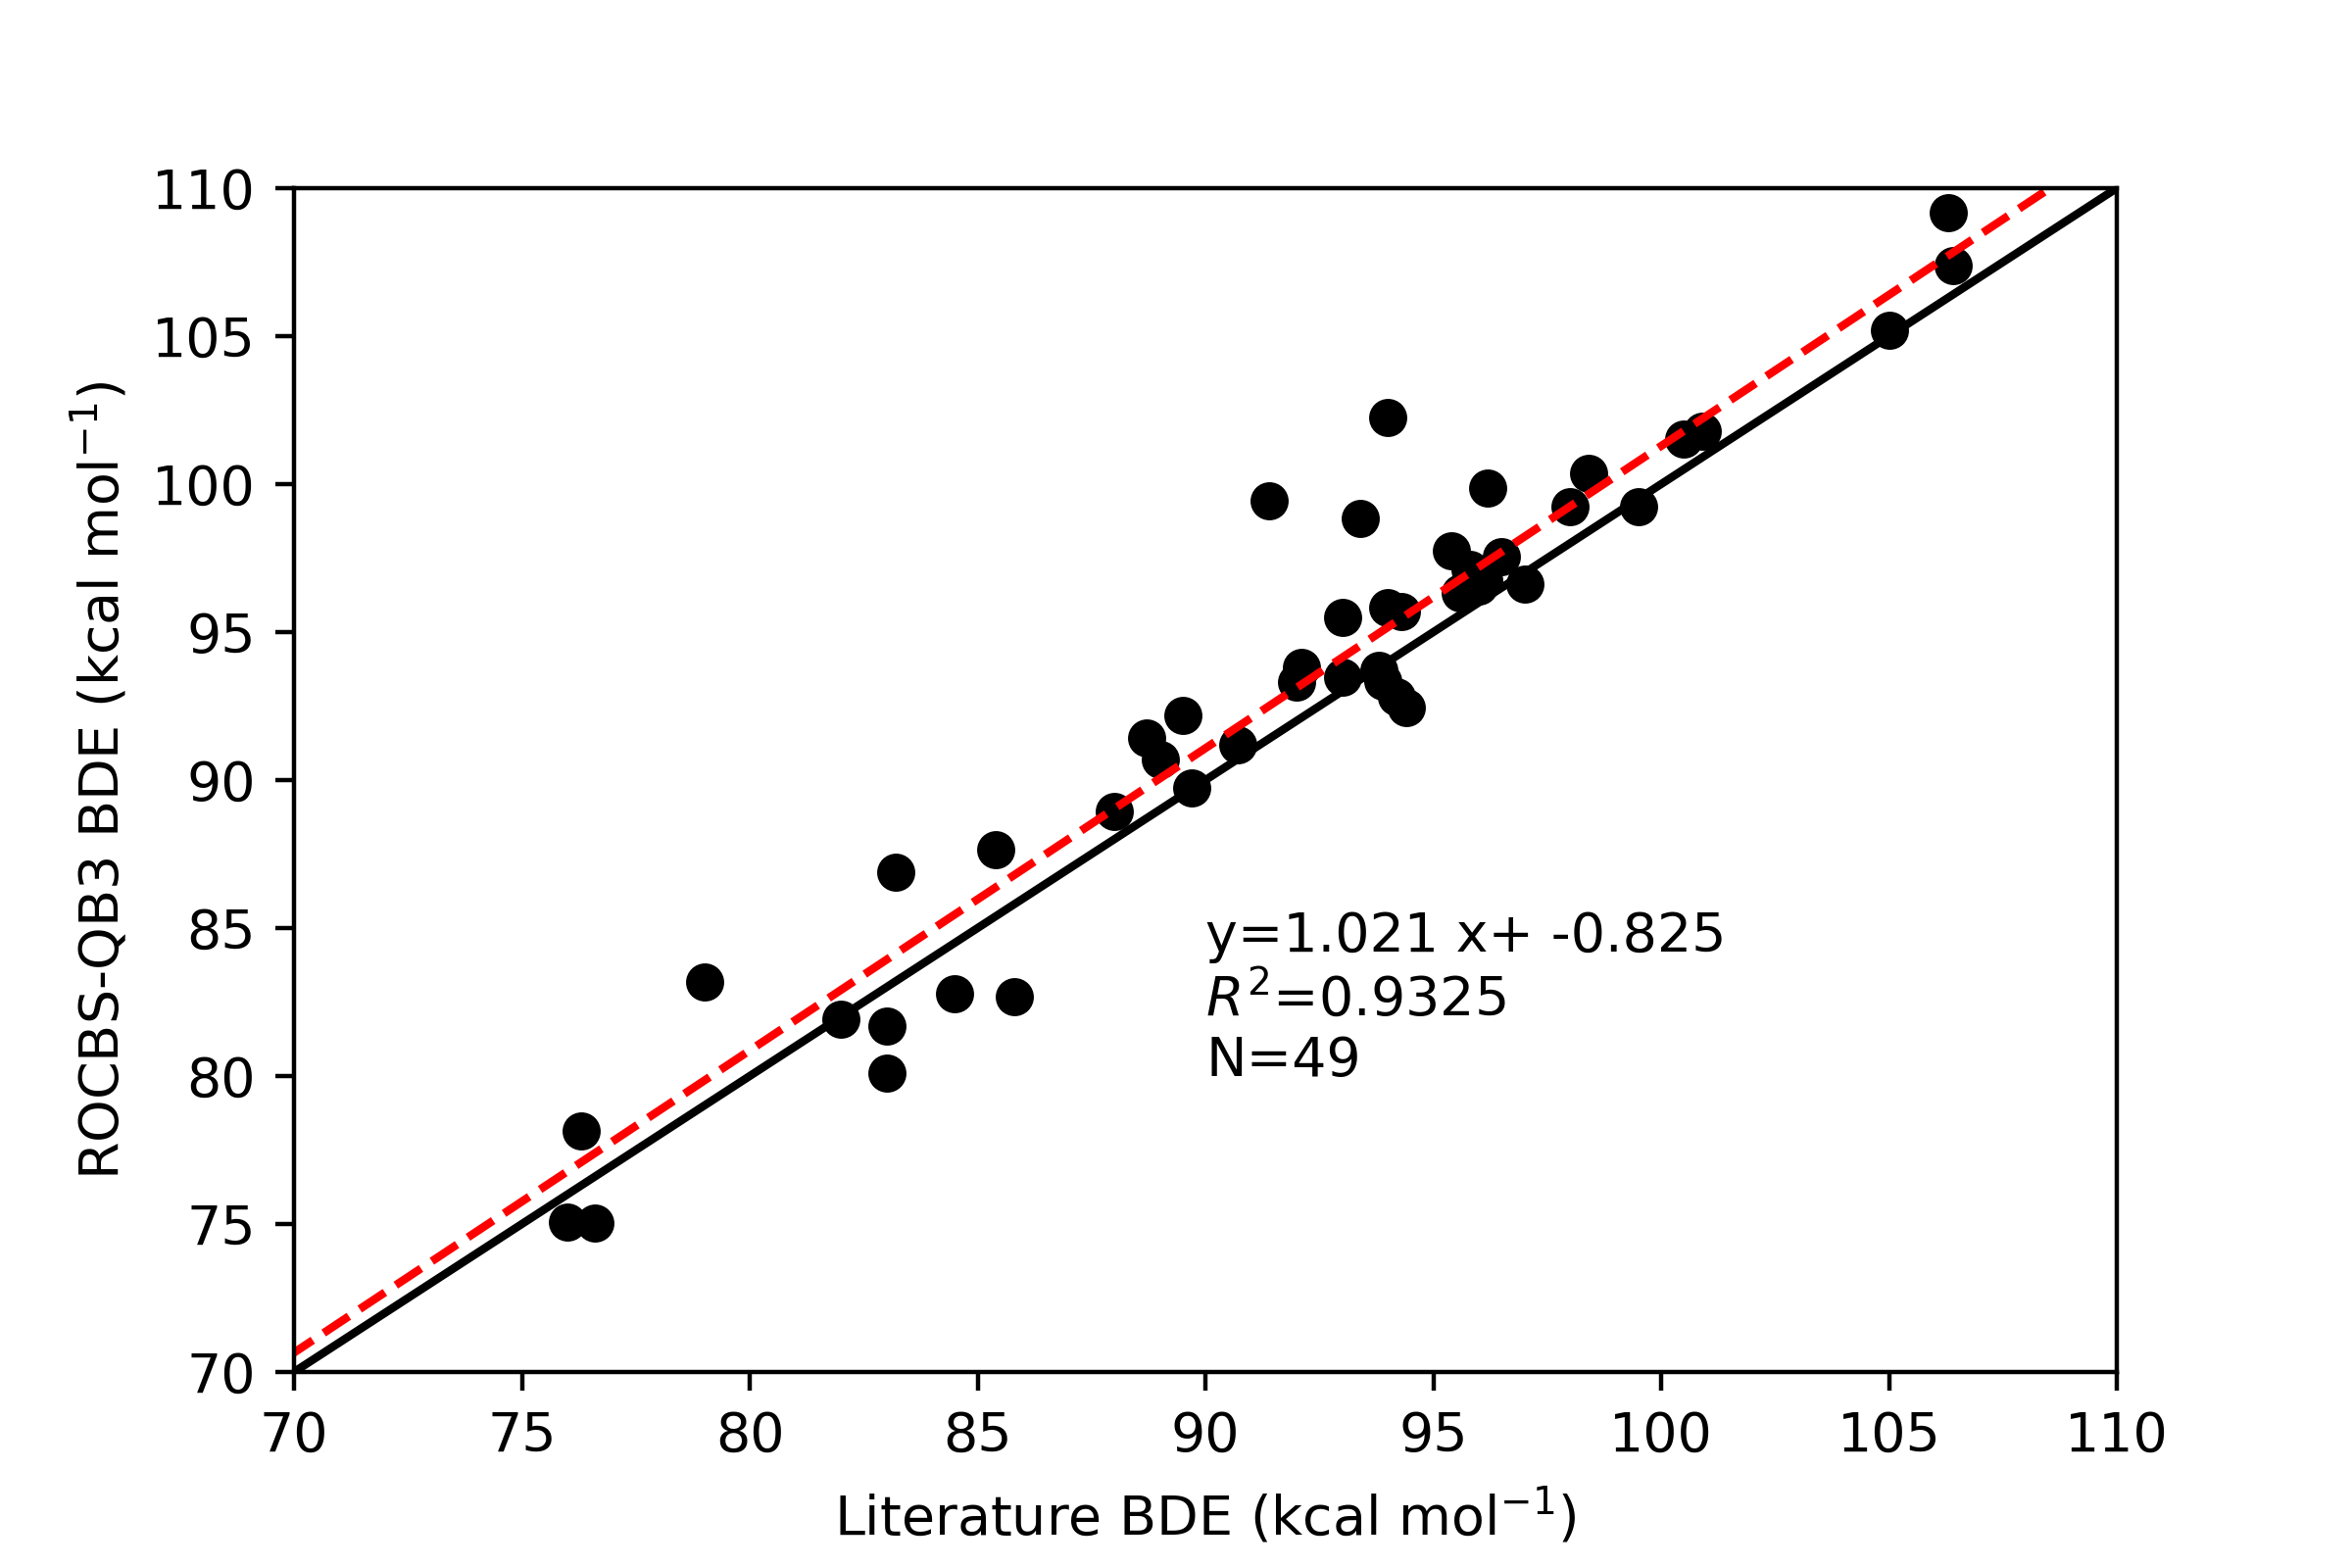
\includegraphics[width=\textwidth]{figures/lit-rocbsqb3}
\end{minipage}
\end{figure}

\begin{figure}
\centering
\begin{minipage}{8cm}
  \centering
  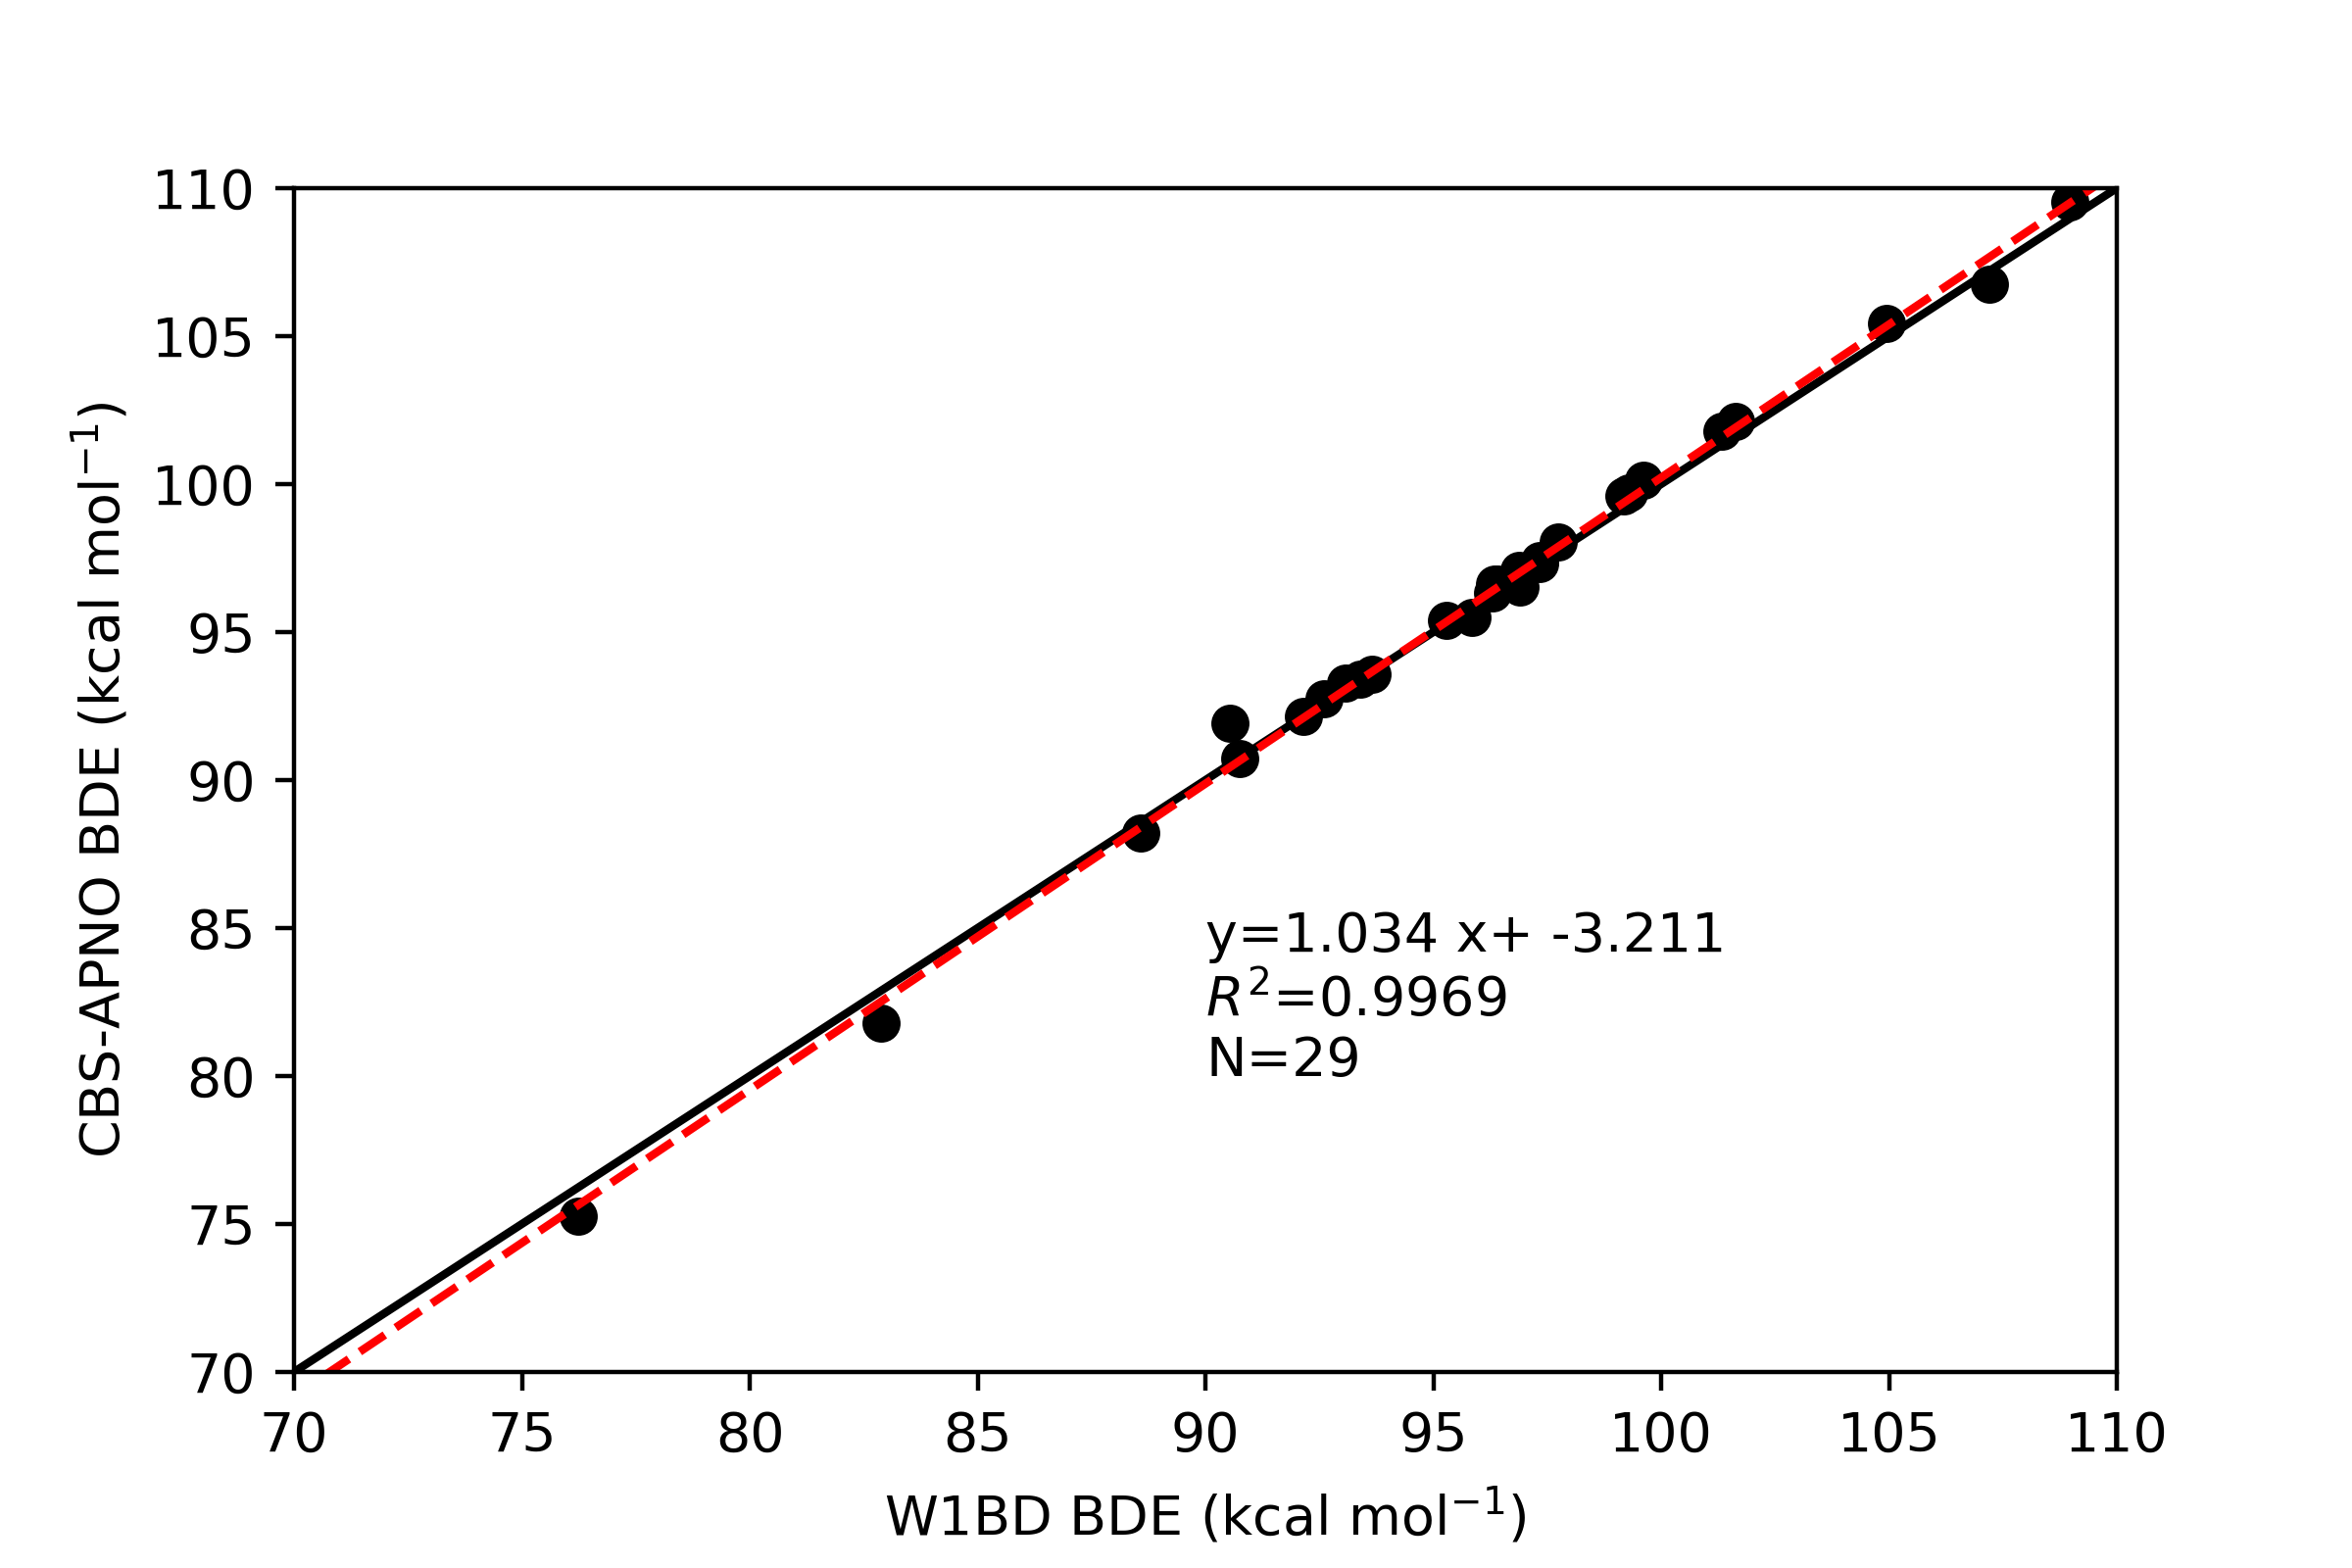
\includegraphics[width=\textwidth]{figures/w1bd-cbsapno}
\end{minipage}%
\begin{minipage}{8cm}
  \centering
  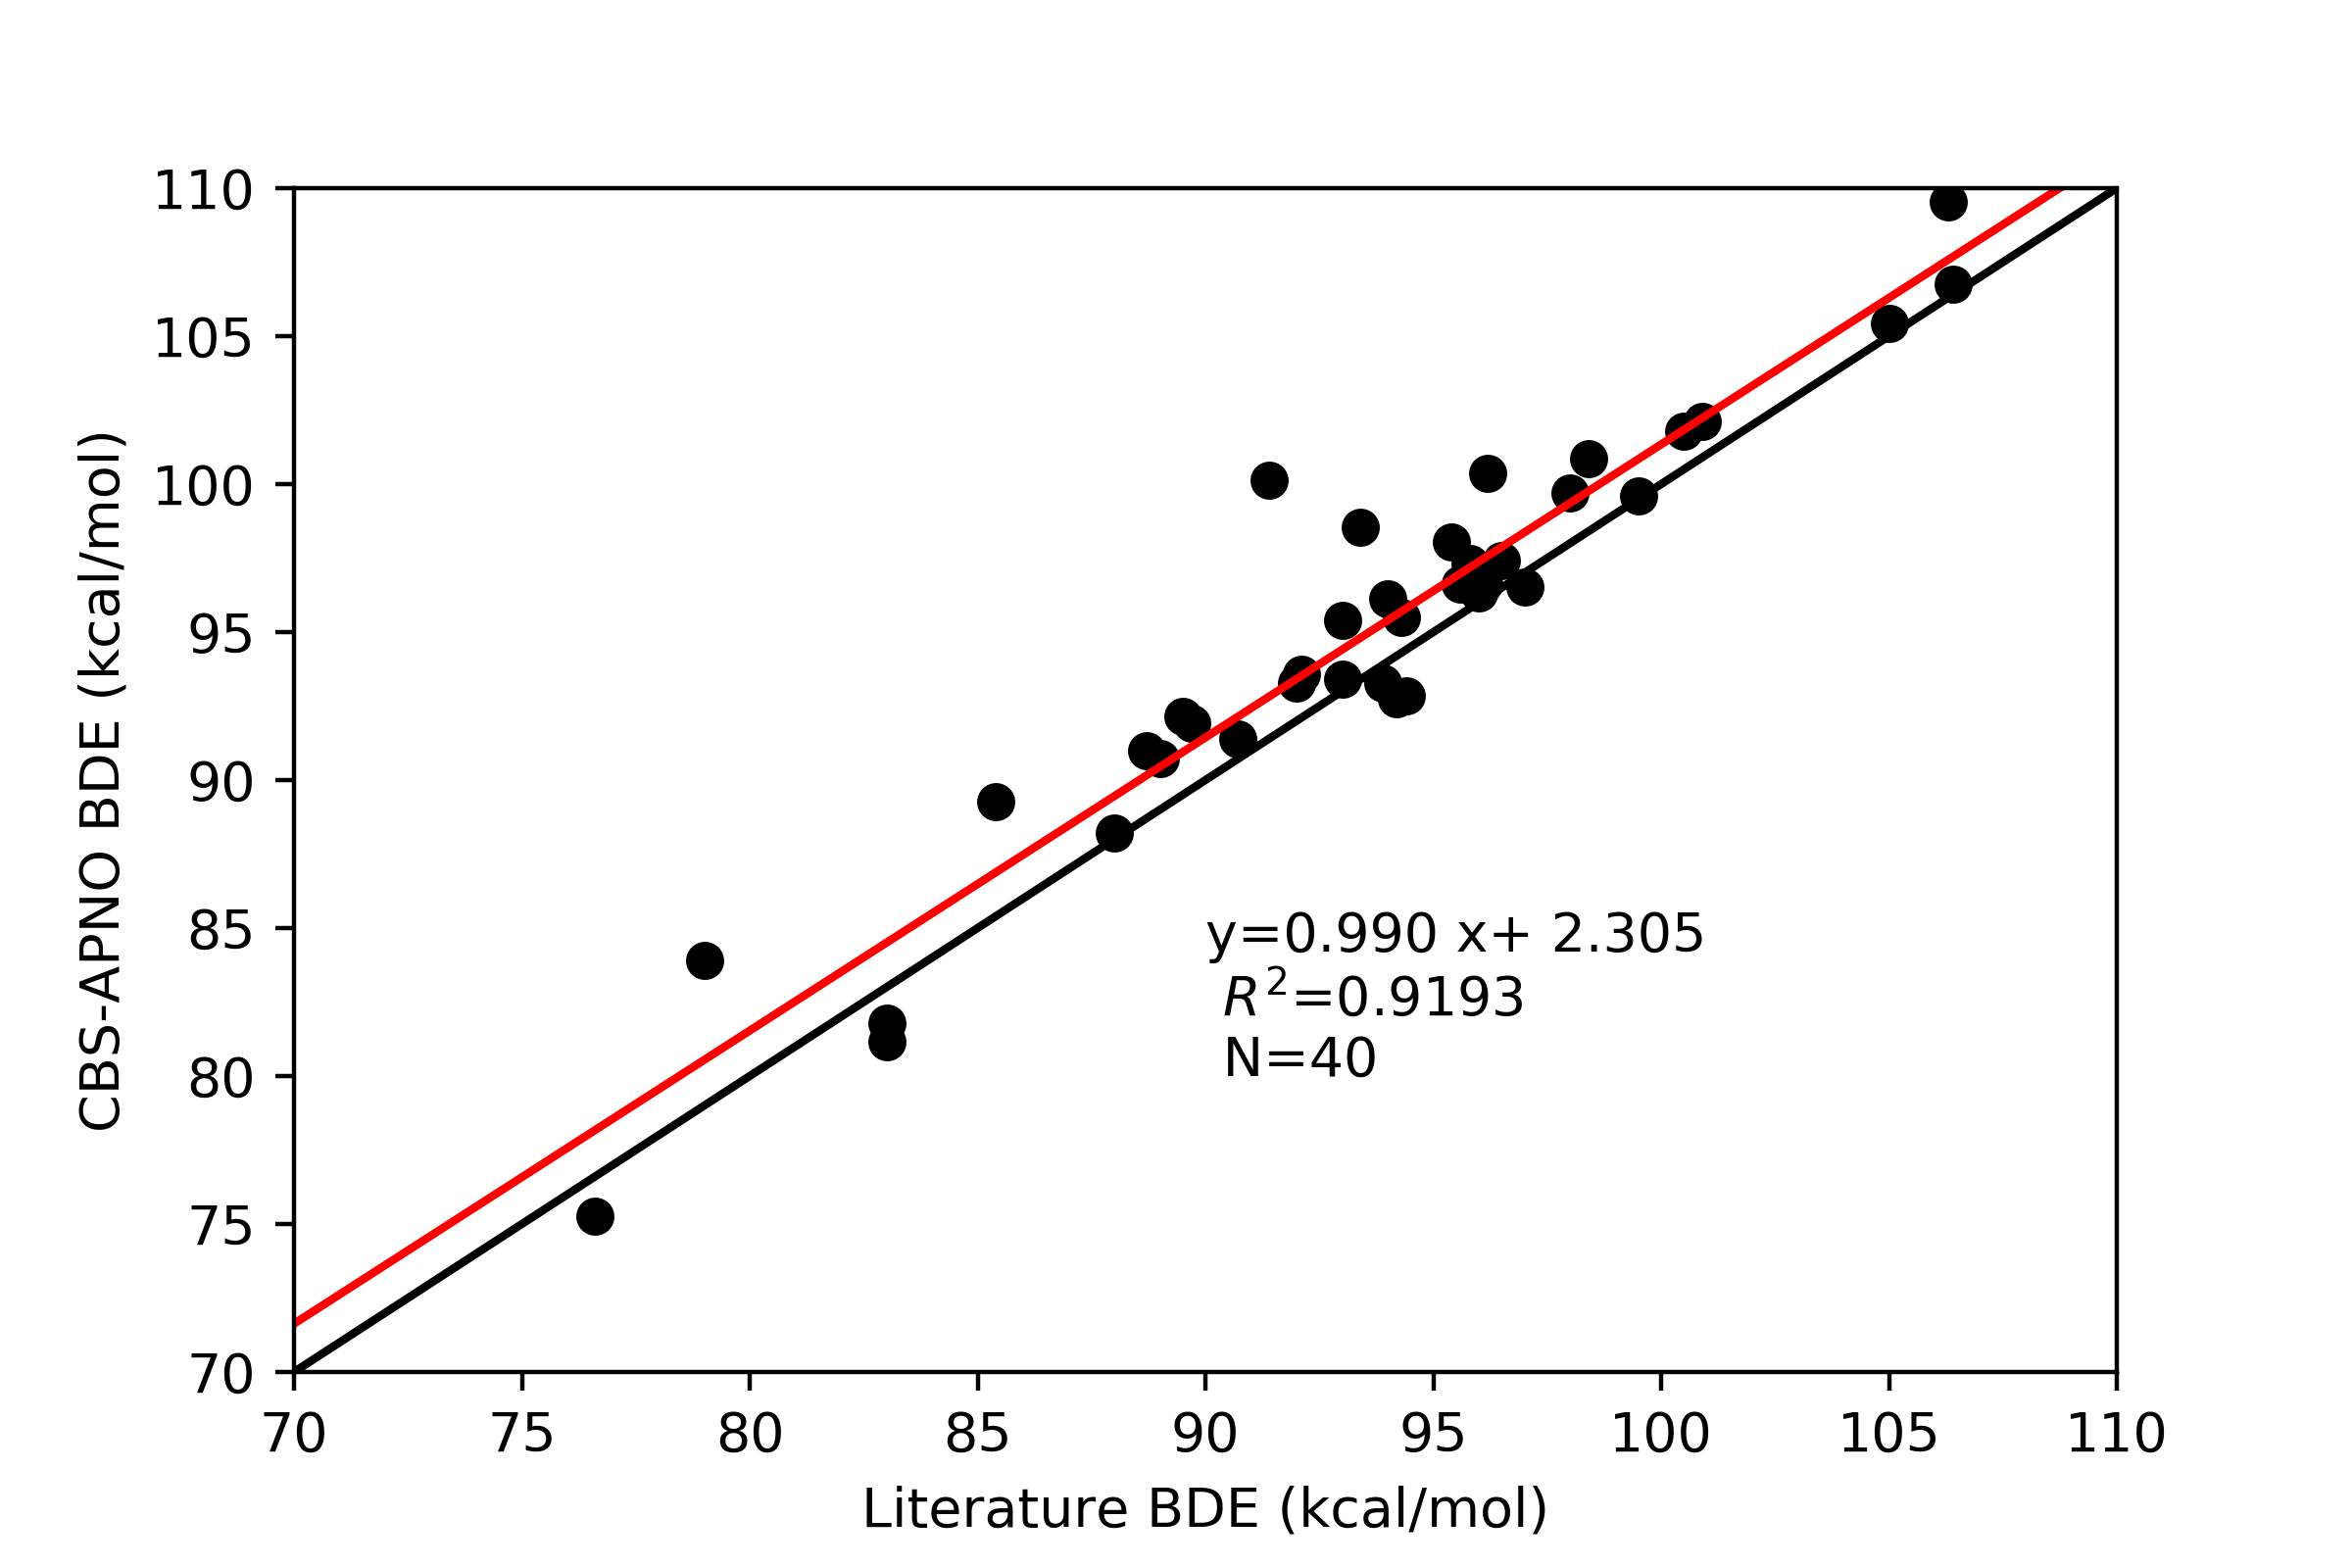
\includegraphics[width=\textwidth]{figures/lit-cbsapno}
\end{minipage}
\end{figure}

\begin{figure}
\centering
\begin{minipage}{8cm}
  \centering
  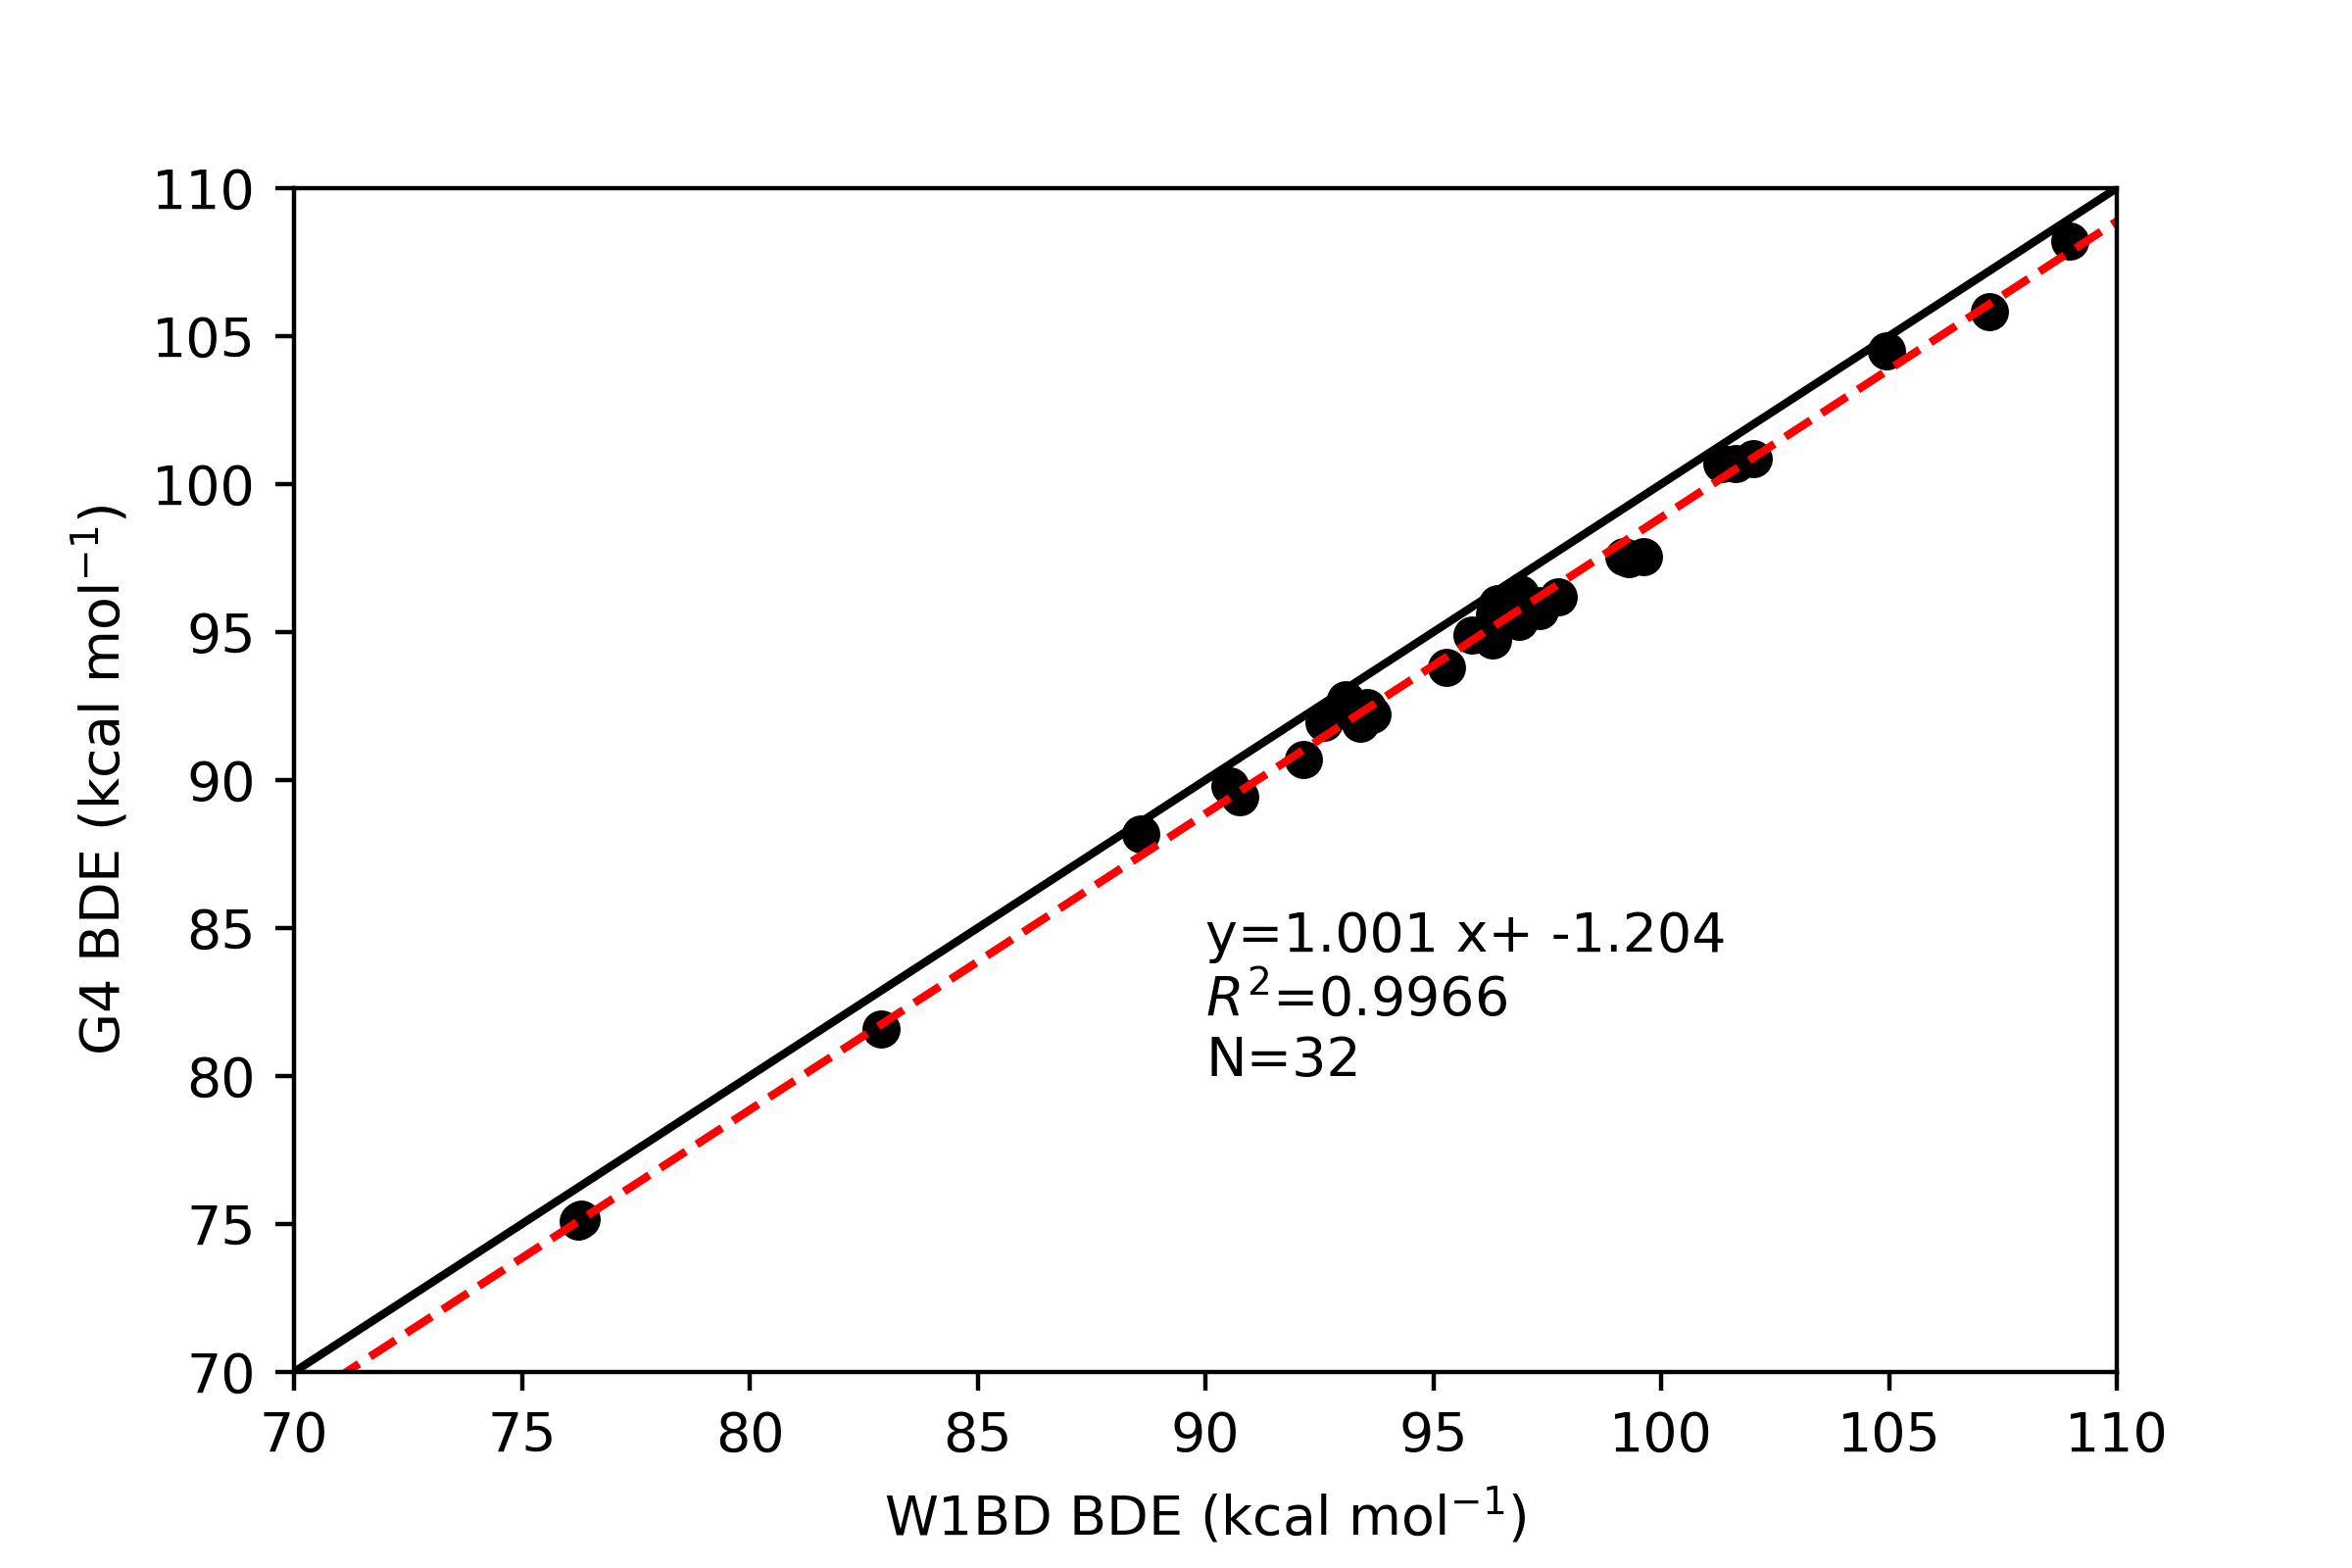
\includegraphics[width=\textwidth]{figures/w1bd-g4}
\end{minipage}%
\begin{minipage}{8cm}
  \centering
  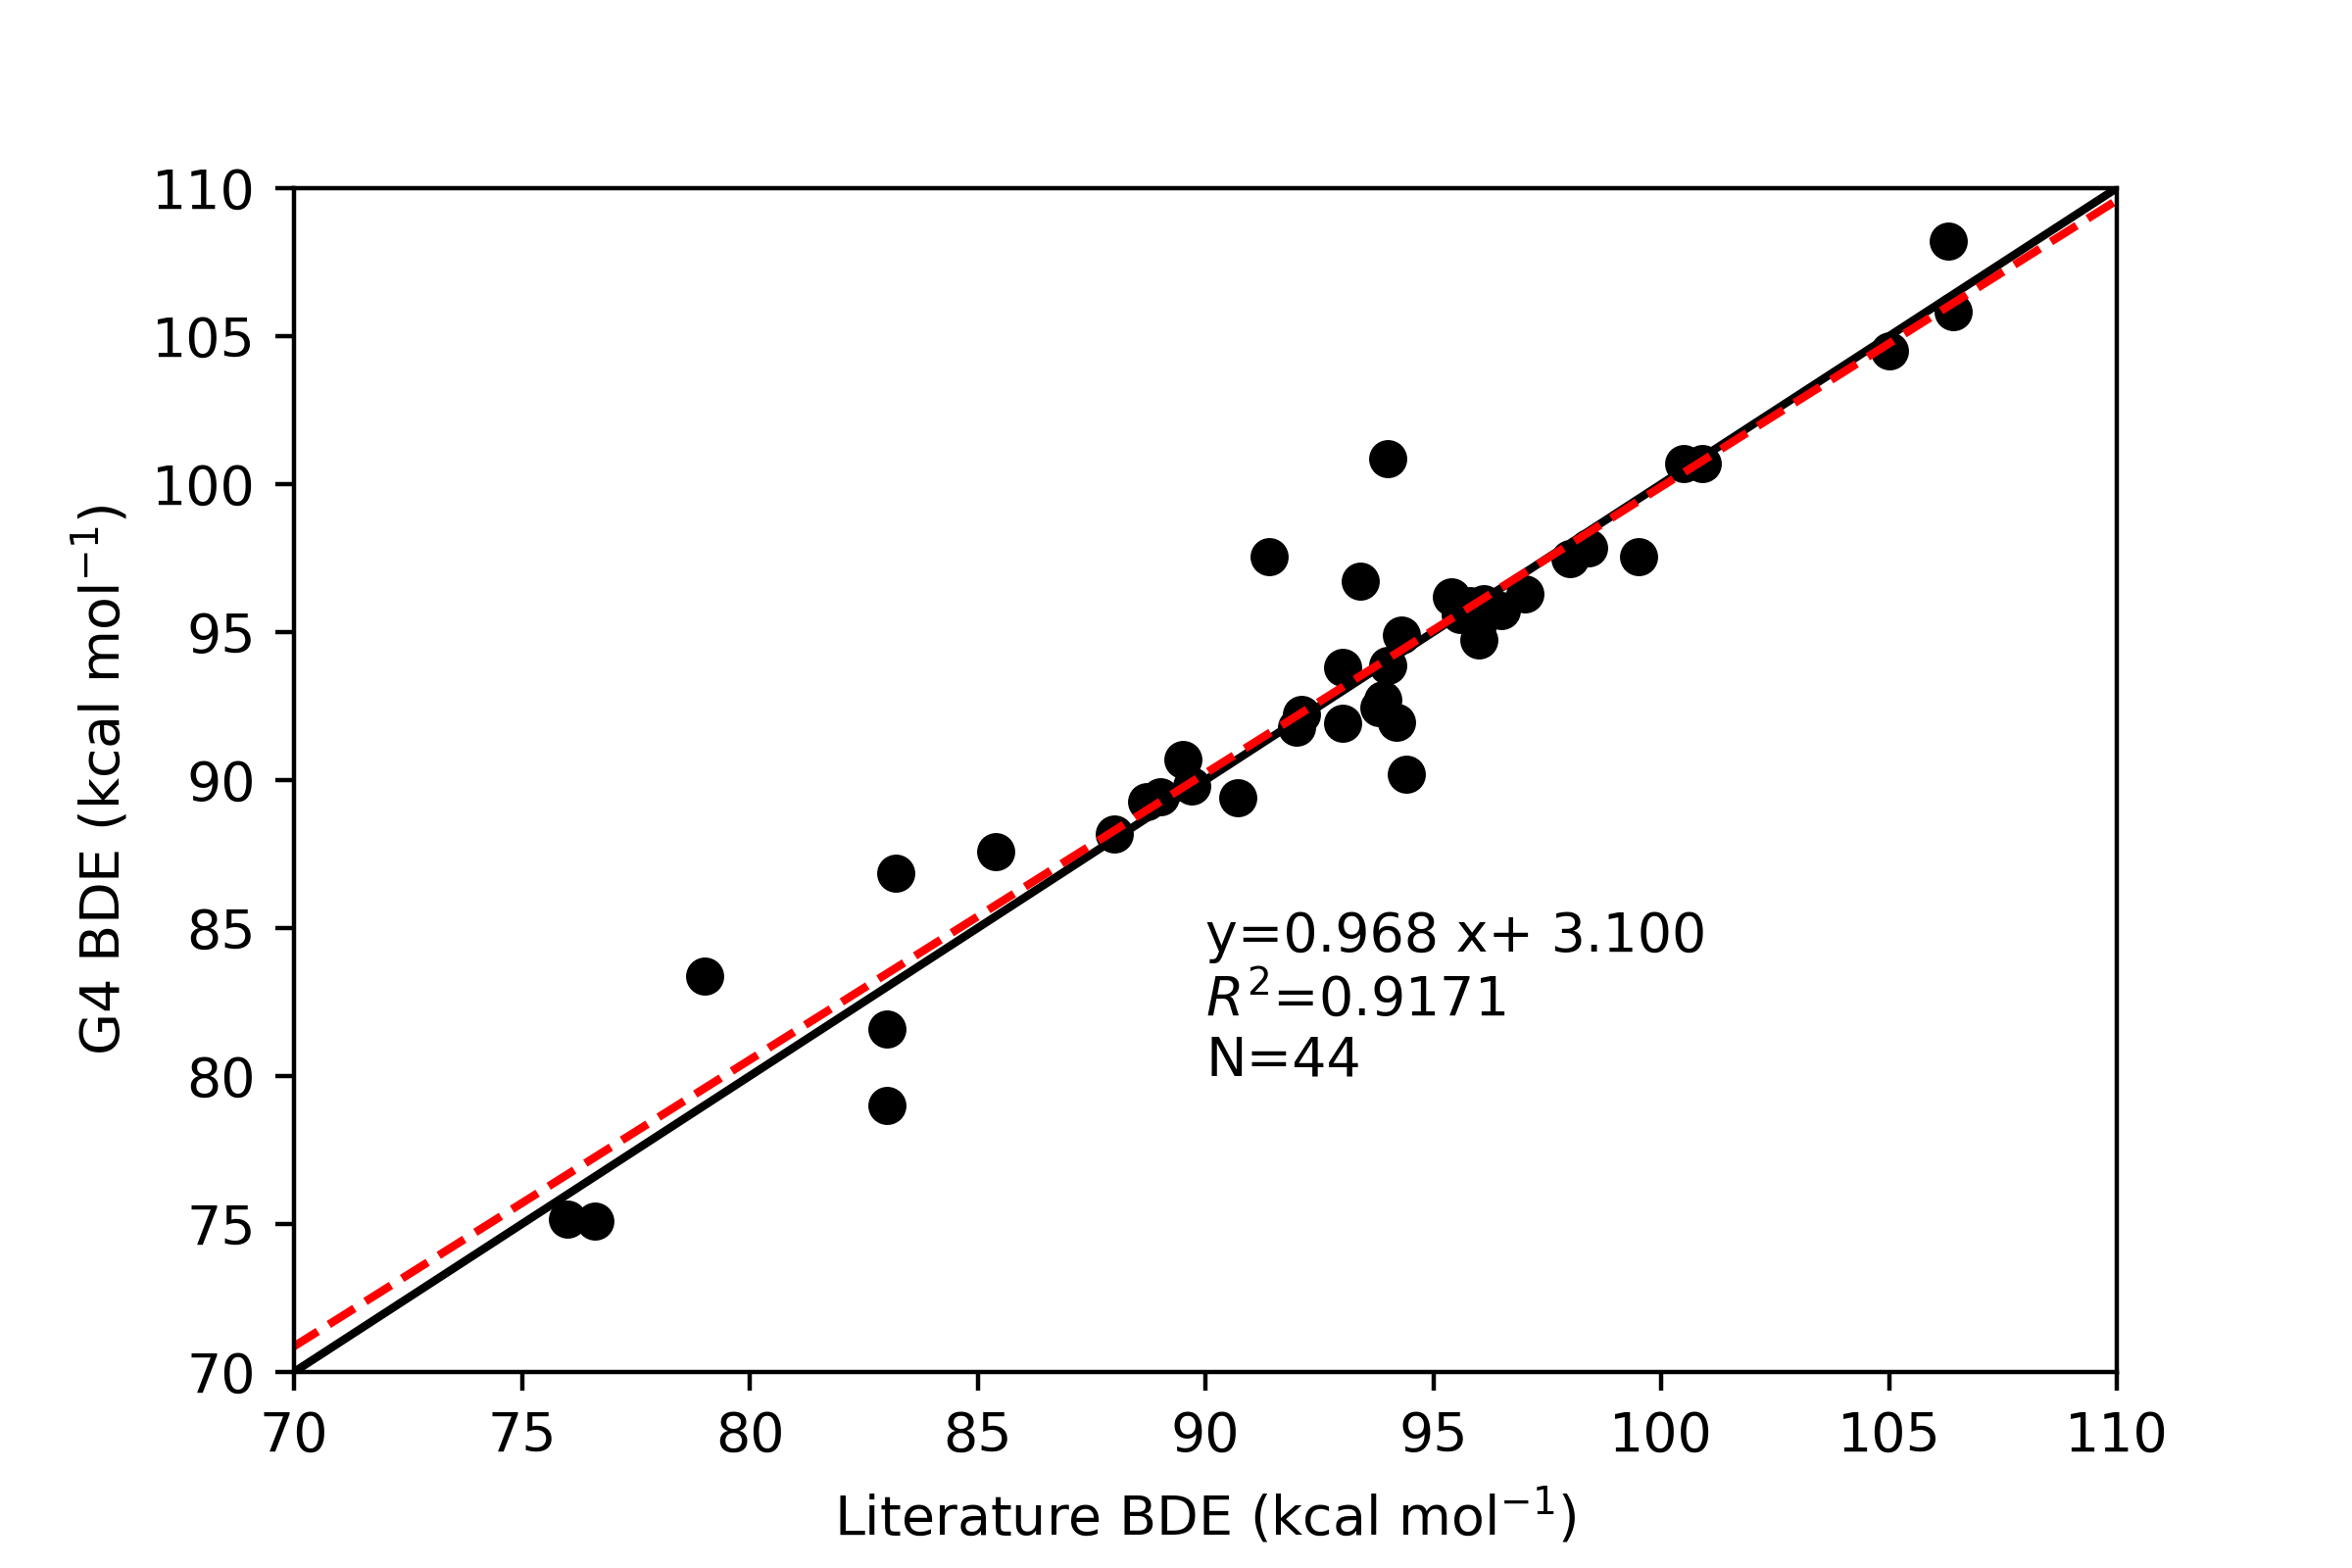
\includegraphics[width=\textwidth]{figures/lit-g4}
\end{minipage}
\end{figure}

\begin{figure}
\centering
\begin{minipage}{8cm}
  \centering
  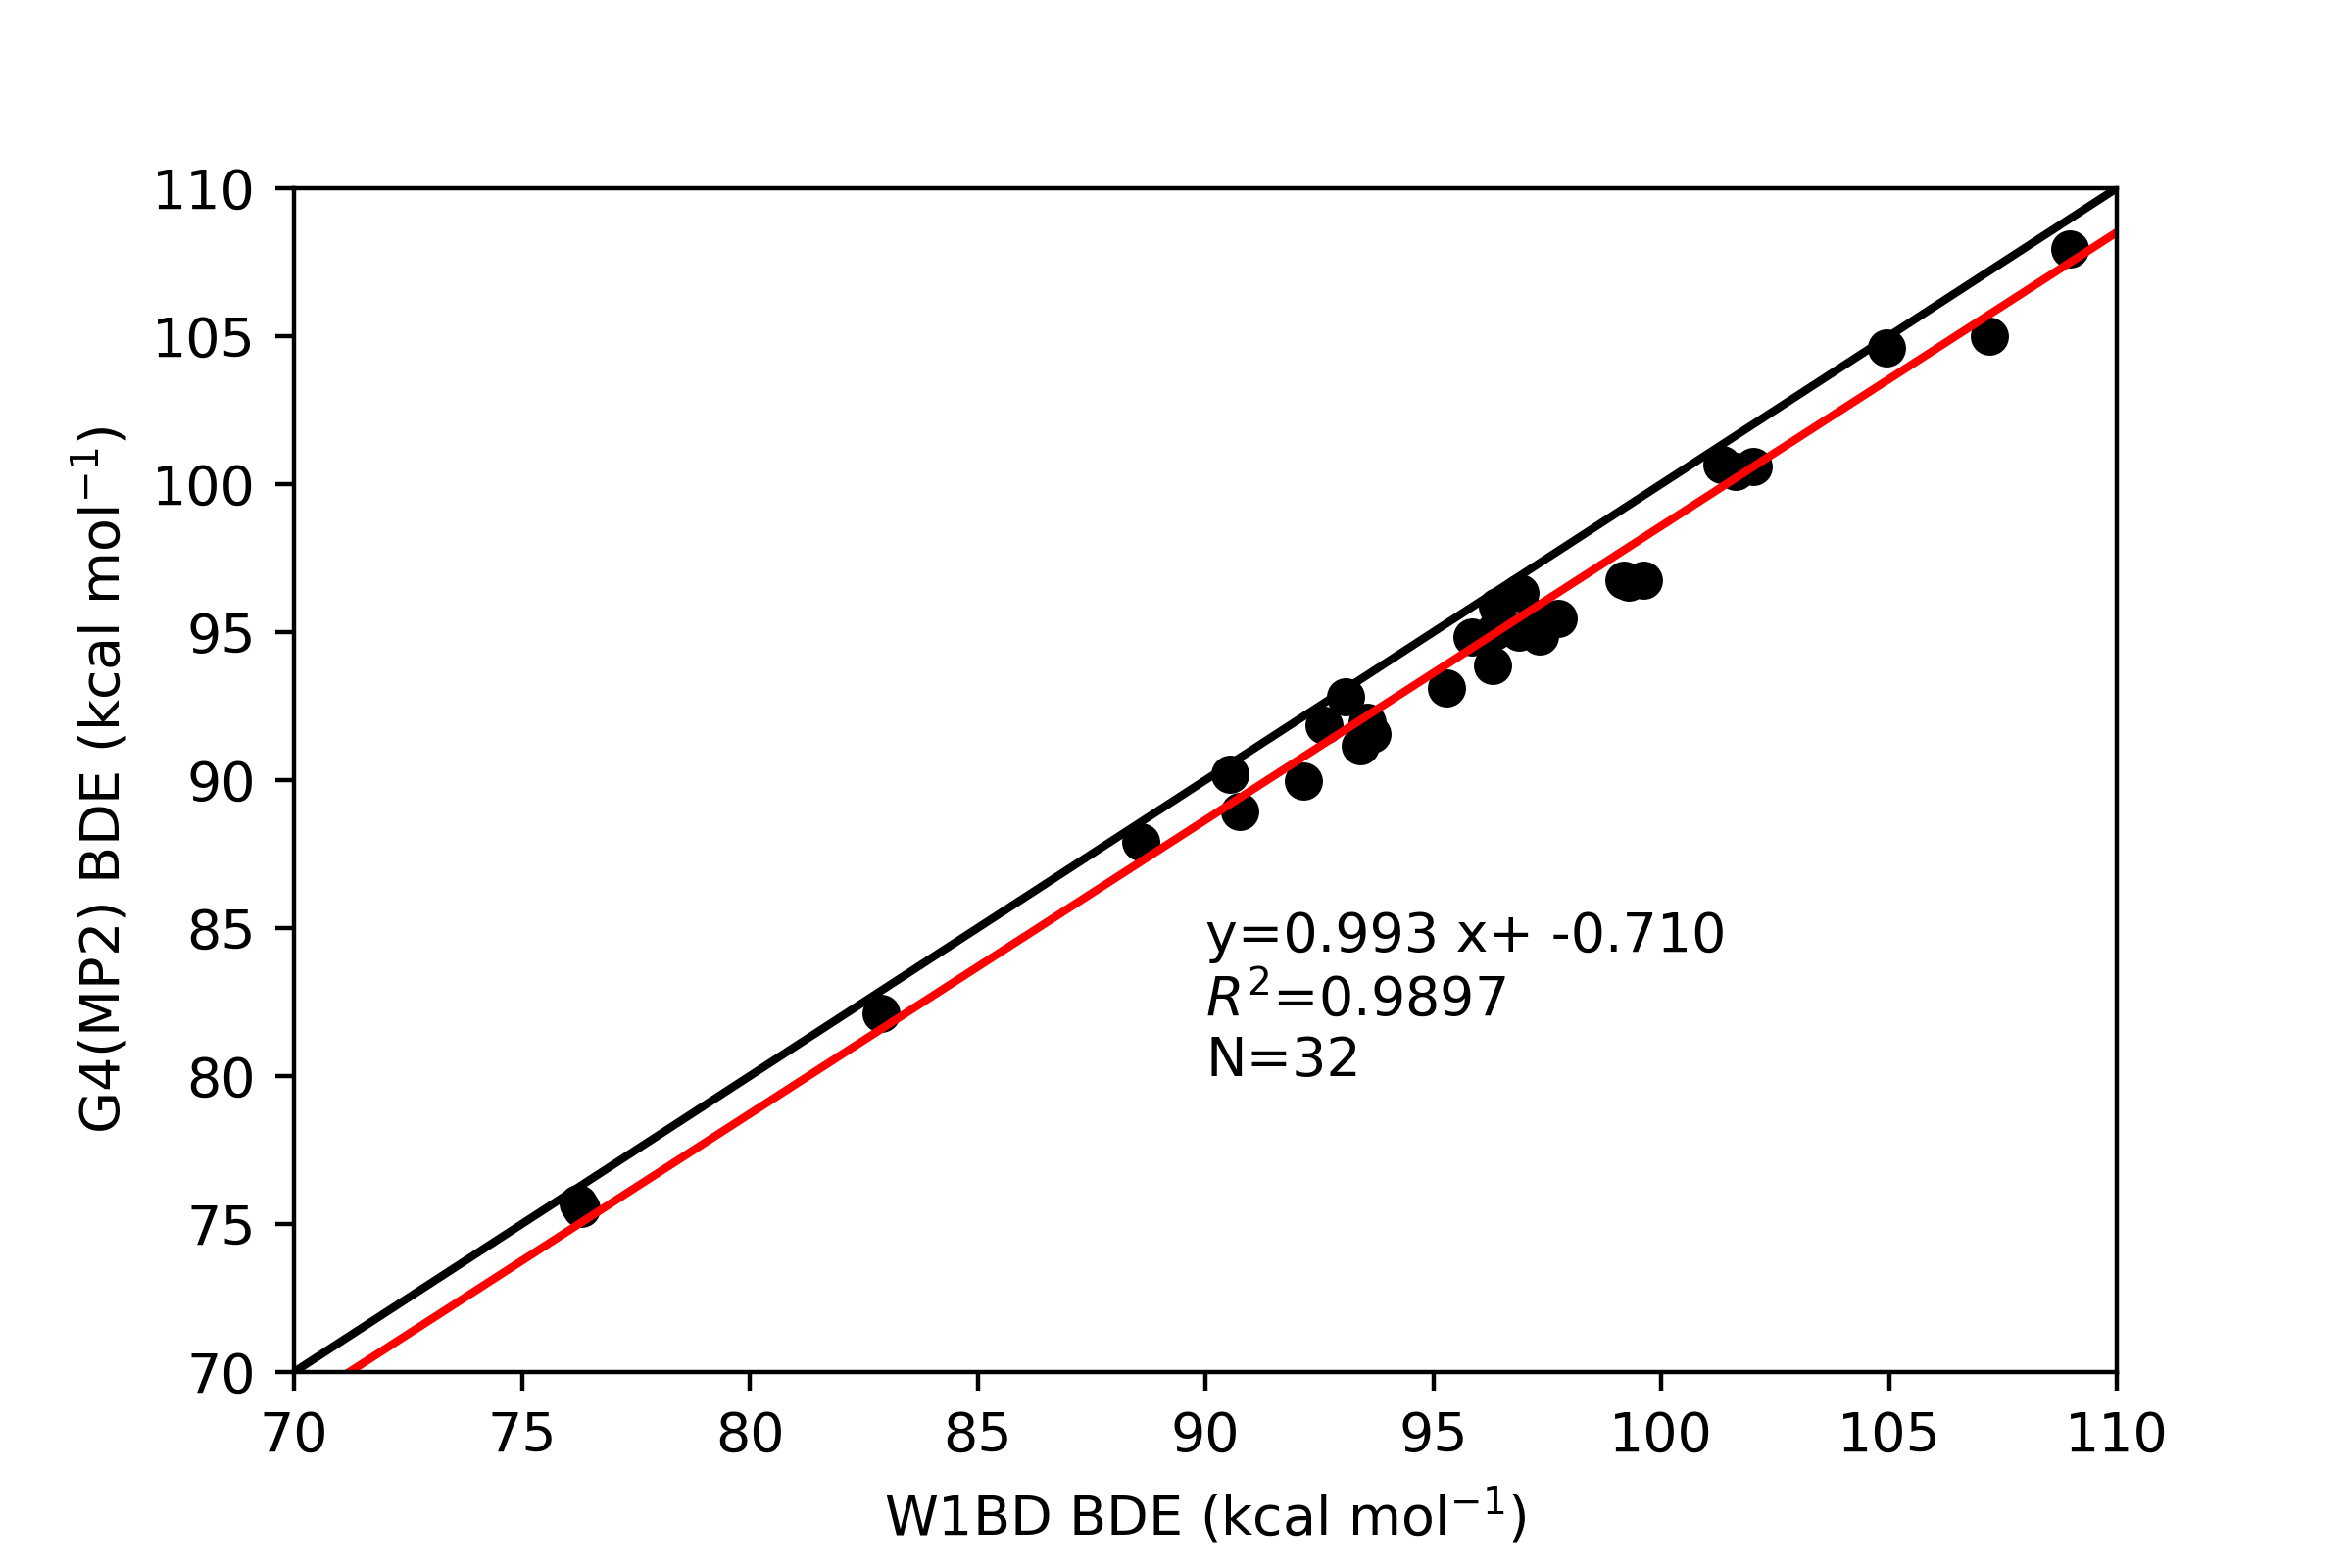
\includegraphics[width=\textwidth]{figures/w1bd-g4mp2}
\end{minipage}%
\begin{minipage}{8cm}
  \centering
  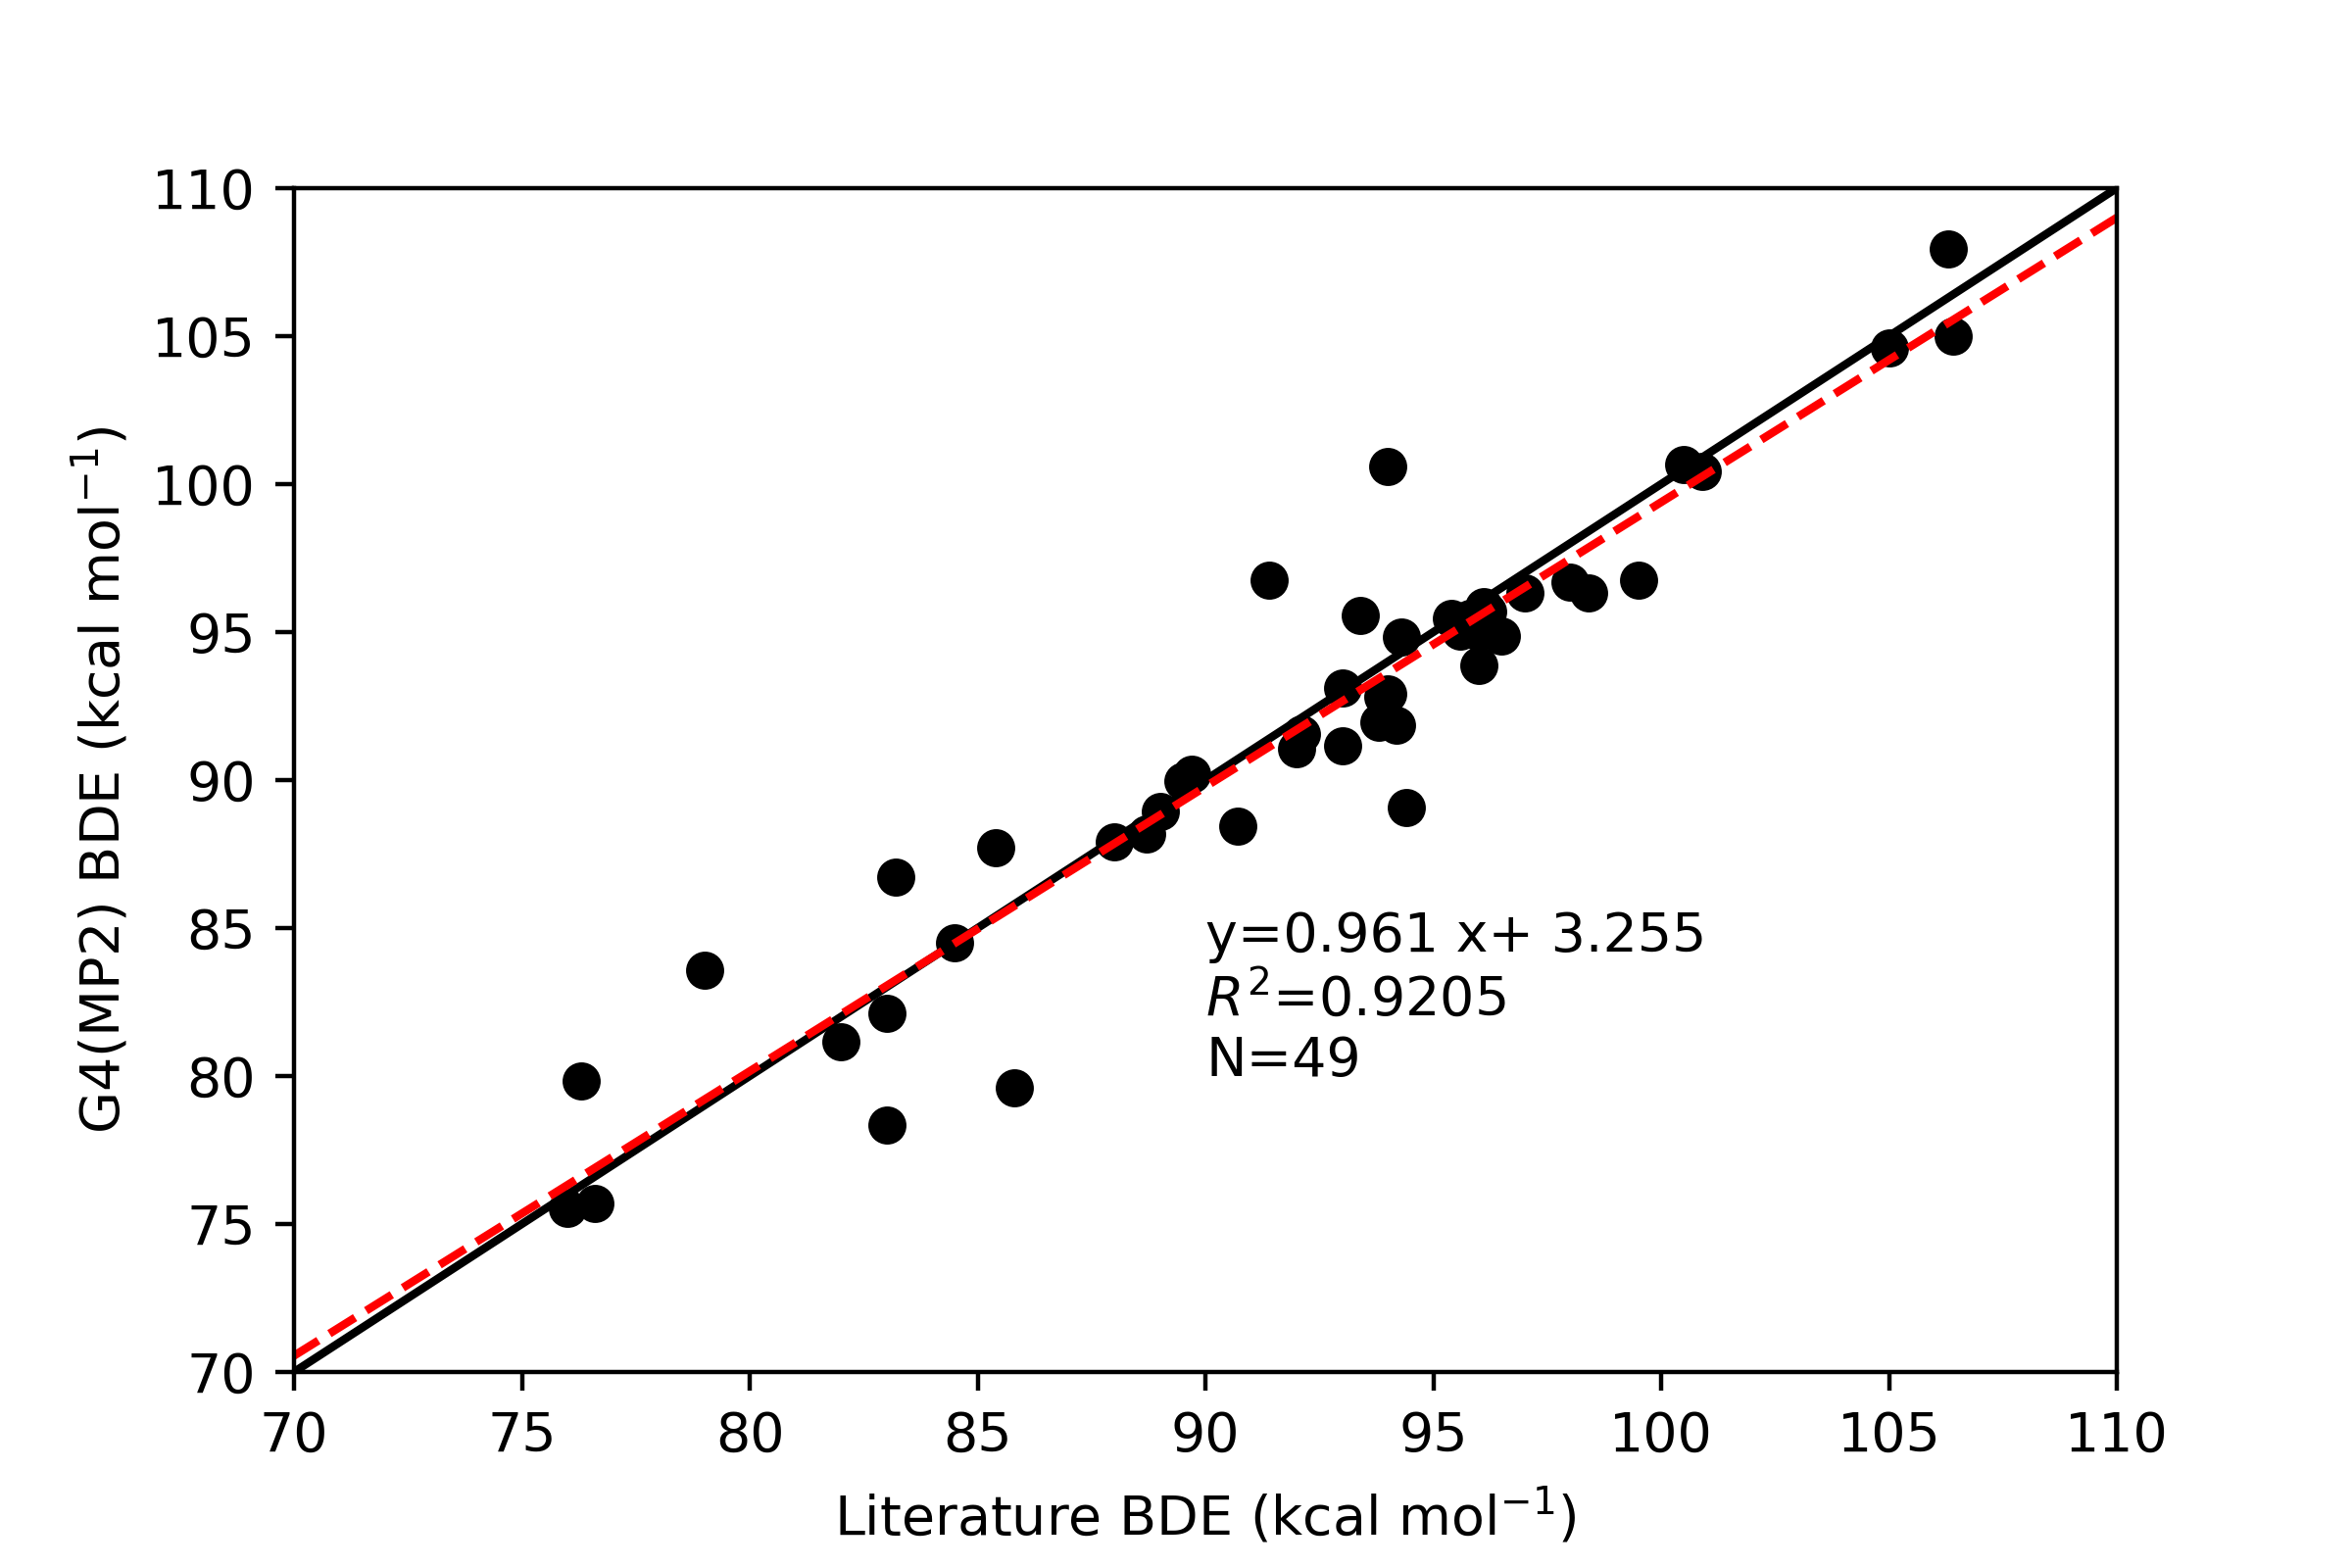
\includegraphics[width=\textwidth]{figures/lit-g4mp2}
\end{minipage}
\end{figure}

\begin{longtable}{m{3.1cm} | c c c}
\caption[Summary of experimental rate constants and literature bond dissociation enthalpies (BDEs).]{Summary of experimental rate constants and literature\cite{Luo2002} bond dissociation enthalpies (BDEs).} \label{tab:expt-bde} \\
\centering
 Molecule                       & $k_H$ \Ms          & Normalized $k_H$ \Ms & BDE \kcalmol \\
\toprule
 1,4-cyclohexadiene             & $ 6.60 \times 10^7$ & $1.65 \times 10^7 $ &        76 \\
 1,4-diazabicyclo-[2.2.2]octane  & $ 9.60 \times 10^6$ & $8.00 \times 10^5 $ &      93.4 \\
 2,2-dimethylbutane             & $ 9.50 \times 10^4$ & $4.75 \times 10^4 $ &        98 \\
 2,3-dimethylbutane             & $ 5.60 \times 10^5$ & $2.80 \times 10^5 $ &      95.4 \\
 9,10-dihydroanthracene         & $ 5.04 \times 10^7$ & $1.26 \times 10^7 $ &      76.3 \\
 Acetone                        & $ < 1 \times 10^4 $ & $2 \times 10^3    $ &        96 \\
 Acetonitrile                   & $ < 1 \times 10^4 $ & $2 \times 10^3    $ &        97 \\
 Adamantane (2$^\circ$)                & $ 6.90 \times 10^6$ & $5.75 \times 10^5 $ &      98.4 \\
 Adamantane (3$^\circ$)                & $ 6.90 \times 10^6$ & $1.73 \times 10^6 $ &      96.2 \\
 Benzaldehyde                   & $ 1.20 \times 10^7$ & $1.20 \times 10^7 $ &      88.7 \\
 Benzyl alcohol                 & $ 2.97 \times 10^6$ & $1.49 \times 10^6 $ &        79 \\
 Cumene                         & $ 5.60 \times 10^5$ & $5.60 \times 10^5 $ &      83.2 \\
 Cycloheptane                   & $ 2.20 \times 10^6$ & $1.57 \times 10^5 $ &        94 \\
 Cyclohexane                    & $ 1.10 \times 10^6$ & $9.17 \times 10^4 $ &      99.5 \\
 Cyclooctane                    & $ 2.98 \times 10^6$ & $1.86 \times 10^5 $ &      94.4 \\
 Cyclopentane                   & $ 9.54 \times 10^6$ & $9.54 \times 10^5 $ &      95.6 \\
 Dibenzyl ether                 & $ 5.60 \times 10^6$ & $1.40 \times 10^6 $ &      85.8 \\
 Diethyl ether                  & $ 2.60 \times 10^6$ & $6.50 \times 10^5 $ &        93 \\
 Dimethyl sulfoxide              & $ 1.80 \times 10^4$ & $6.00 \times 10^3 $ &        94 \\
 Dioxane                        & $ 8.20 \times 10^5$ & $1.03 \times 10^5 $ &      96.5 \\
 Diphenylmethane                & $ 8.71 \times 10^5$ & $4.36 \times 10^5 $ &      84.5 \\
 Ethylbenzene                   & $ 7.90 \times 10^5$ & $3.95 \times 10^5 $ &      85.4 \\
 Hexamethyl-phorsphoramide       & $ 1.87 \times 10^7$ & $1.04 \times 10^6 $ &           \\
 Morpholine                     & $ 5.00 \times 10^7$ & $1.25 \times 10^7 $ &        92 \\
 Piperazine                     & $ 2.4 \times 10^8 $ &                &        93 \\
 Piperidine                     & $ 1.2 \times 10^8 $ &                &      89.5 \\
 Pyrrolidine                    & $ 1.1 \times 10^8 $ &                &        89 \\
 Tetrahydro-2H-pyran            & $ 1.4 \times 10^6 $ &                &        96 \\
 Tetrahydrofuran                & $ 5.8 \times 10^6 $ &                &      92.1 \\
 Toluene                        & $ 1.85 \times 10^5$ & $6.17 \times 10^4 $ &      89.7 \\
 Triethylamine                  & $ 2.10 \times 10^8$ & $3.5 \times 10^7  $ &      90.7 \\
 Triphenylmethane               & $ 3.04 \times 10^5$ & $3.04 \times 10^5 $ &        81 \\
\end{longtable}

